%!TEX root = thesis.tex

\begin{appendices}
\chapter{List Of Symbols}
\begin{tabular}{cp{\textwidth}}
  $x$ & Location, spatial or spatio-temporal \\
  $w$ & Word, an instance of a discrete-valued feature ($\textbf{w}$, all words) \\
  $z$ & Topic assignment ($\textbf{z}$, all topic assignments) \\
  $g(x)$ & The neighborhood of location $x$ \\
  $g$ & Parameter controlling neighborhood size \\
  $\theta$, $\theta_{g(x)}$ & Topic prior for one neighborhood ($\Theta$, all topic priors)\\
  $\phi$, $\phi_k$ & Word distribution for one topic ($\Phi$, all topics) \\
  $\alpha$ & Parameter of symmetric Dirichlet prior on $\theta$ \\
  $\beta$ & Parameter of symmetric Dirichlet prior on $\phi$ \\
  $K$ & Number of topics \\
  $V$ & Vocabulary size, number of distinct values of $w$ \\
  $N_{g(x)}^k$ & Number of times topic $k$ was used in neighborhood $g(x)$ \\
  $N_k^v$ & Number of times topic $k$ was used for word $v$ \\
  $N_{\cdot,-i}^\cdot$ & Count as above, but excluding the $i$-th datapoint\\
  $\sigma$ & The softmax function where the $i$-th dimension $\sigma(x)_i = {e^{x_i}} / \sum_j e^{x_j}$
\end{tabular}\\

\chapter{Categorical Information Boost Autoencoder Architecture Details} \label{ch:cibae-arch}
Similar to Segnet \citep{BadrinarayananK15}, our implementation uses a symmetric sequence of downsampling convolution modules (DownConvModule Fig.~\ref{fig:DownConvMod}) and upsampling convolution modules (UpConvModule Fig.~\ref{fig:UpConvMod}), where the spatial resolution changes by a factor of two at the end of each module. All convolutions are with kernel size 3, stride 1, and padding 1 so that the input and output spatial resolutions are identical.

\begin{lstlisting}[language=Python, caption=CIB-AE Architecture Detail, label=cibae_arch]]
CIB_AE(
    Encoder(
        DownConvModule(3, 64, 2),
        DownConvModule(64, 128, 3),
        DownConvModule(128, 256, 3),
        DownConvModule(256, 512, 3),
        DownConvModule(512, 512, 3),
        Reshape((4, 4, 512) -> (8192)),
        Dropout(p=0.25),
        Softmax()
    ), 
    Decoder(
        Reshape((8192) -> (4, 4, 512)),
        UpConvModule(512, 512, 3),
        UpConvModule(512, 256, 3)
        UpConvModule(256, 128, 3),
        UpConvModule(128, 64, 2),
        UpConvModule(64, 3, 2)
    )
)
\end{lstlisting}

In our experiments we found that the single Dropout layer before the Softmax in the encoder was crucial. Without dropout, the encodings become overly sensitive to differences in the input images, and approximate encodings through our topic model and topic mapping algorithms are too different from real encodings to produce reasonable results.

\begin{figure}
    \begin{center}
    \subfloat[]{
        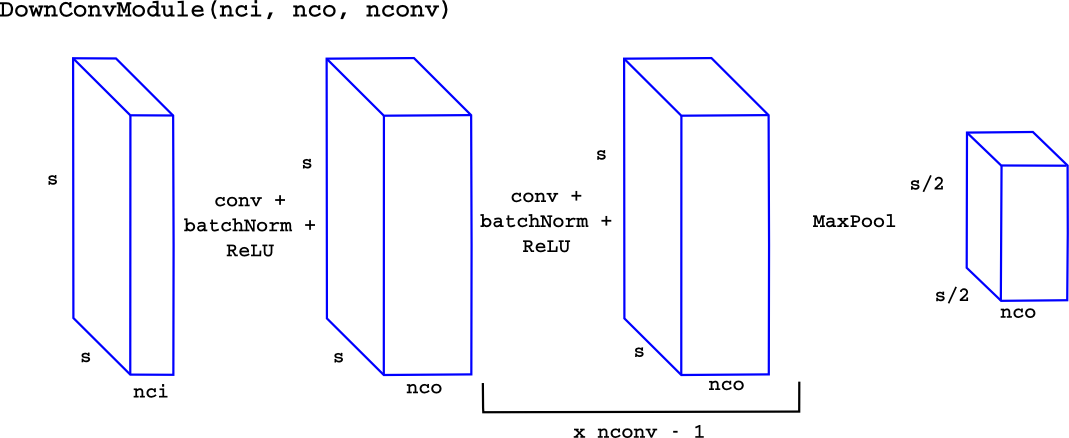
\includegraphics[width=0.8\columnwidth]{figures/ptz/DownConvModule.png}
        \label{fig:DownConvMod}
    }\\
    \subfloat[]{
        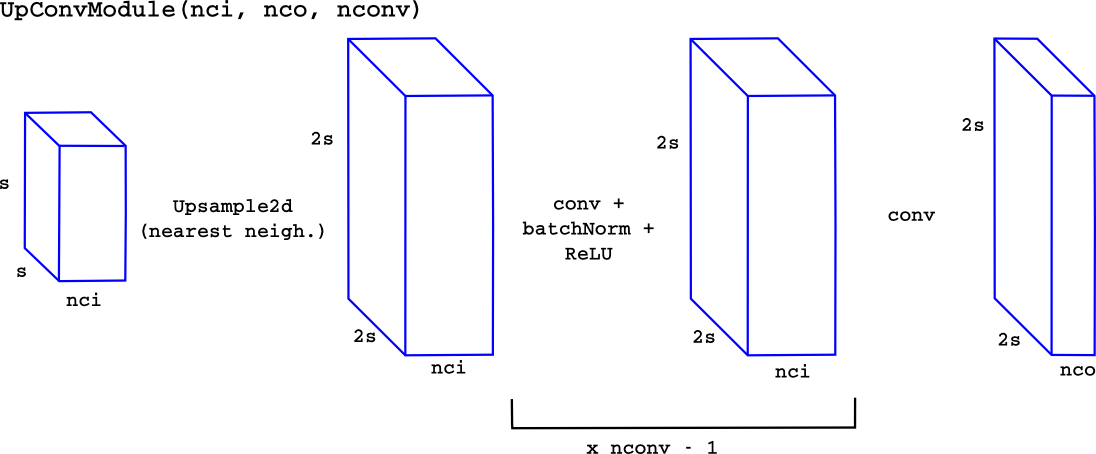
\includegraphics[width=0.8\columnwidth]{figures/ptz/UpConvModule.png}
        \label{fig:UpConvMod}
    }
    \end{center}
    \caption{
    \protect\subref{fig:DownConvMod} DownConv and \protect\subref{fig:UpConvMod} UpConv modules used in our architecture. nci stands for number of channels in, nco number of channels out, and s the spatial resolution of the input representation. In our model, $nco = 2 nci$ for DownConvModules and $nco = nci/2$ for UpConvModules. Each block is made of a sequence of convolution, batch norm, nonlinear activation blocks. The last convolution of the UpConvModule does not include the batch norm and nonlinearities because the training images are standardized (\emph{ie.} pixel values can be both negative and positive).
    }
    \label{fig:cib-ae_modules}
\end{figure}

\chapter{Spatial Image Prediction Examples} \label{ch:app-predictions}
\begin{figure}
    \centering
    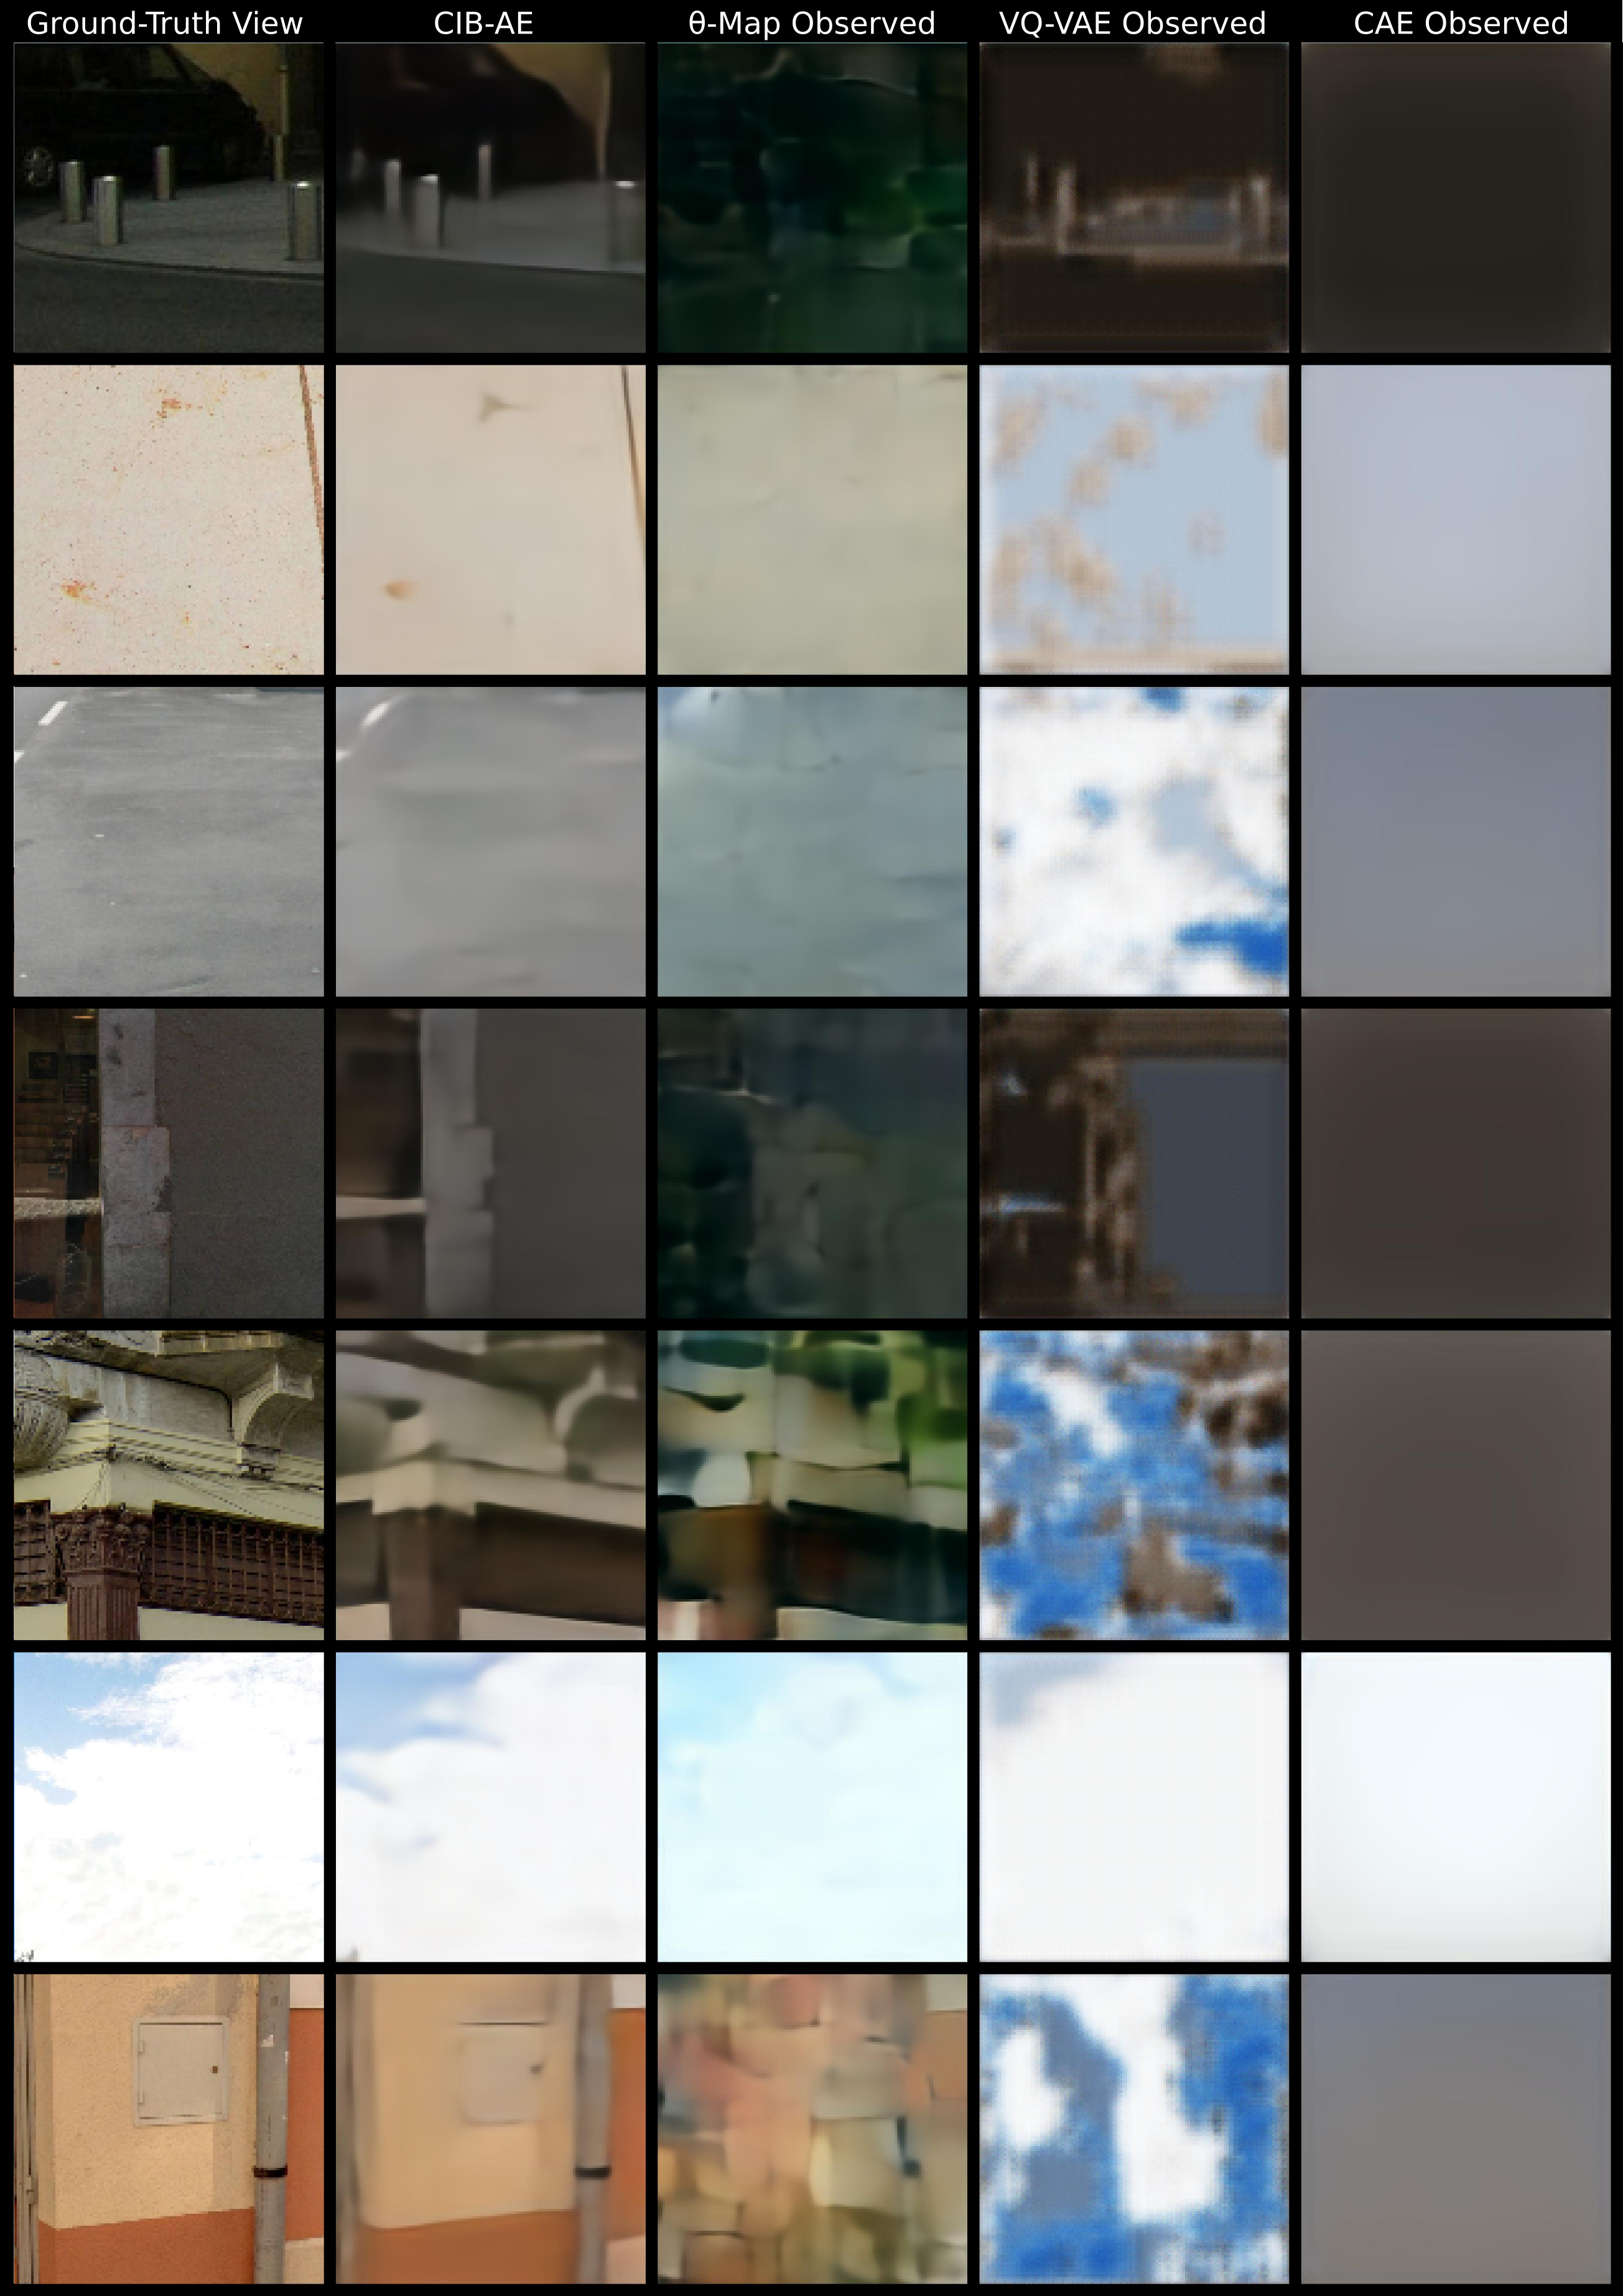
\includegraphics[width=0.92\textwidth]{figures/ptz/train_stacked_0.png}
\end{figure}
\begin{figure}
    \centering
    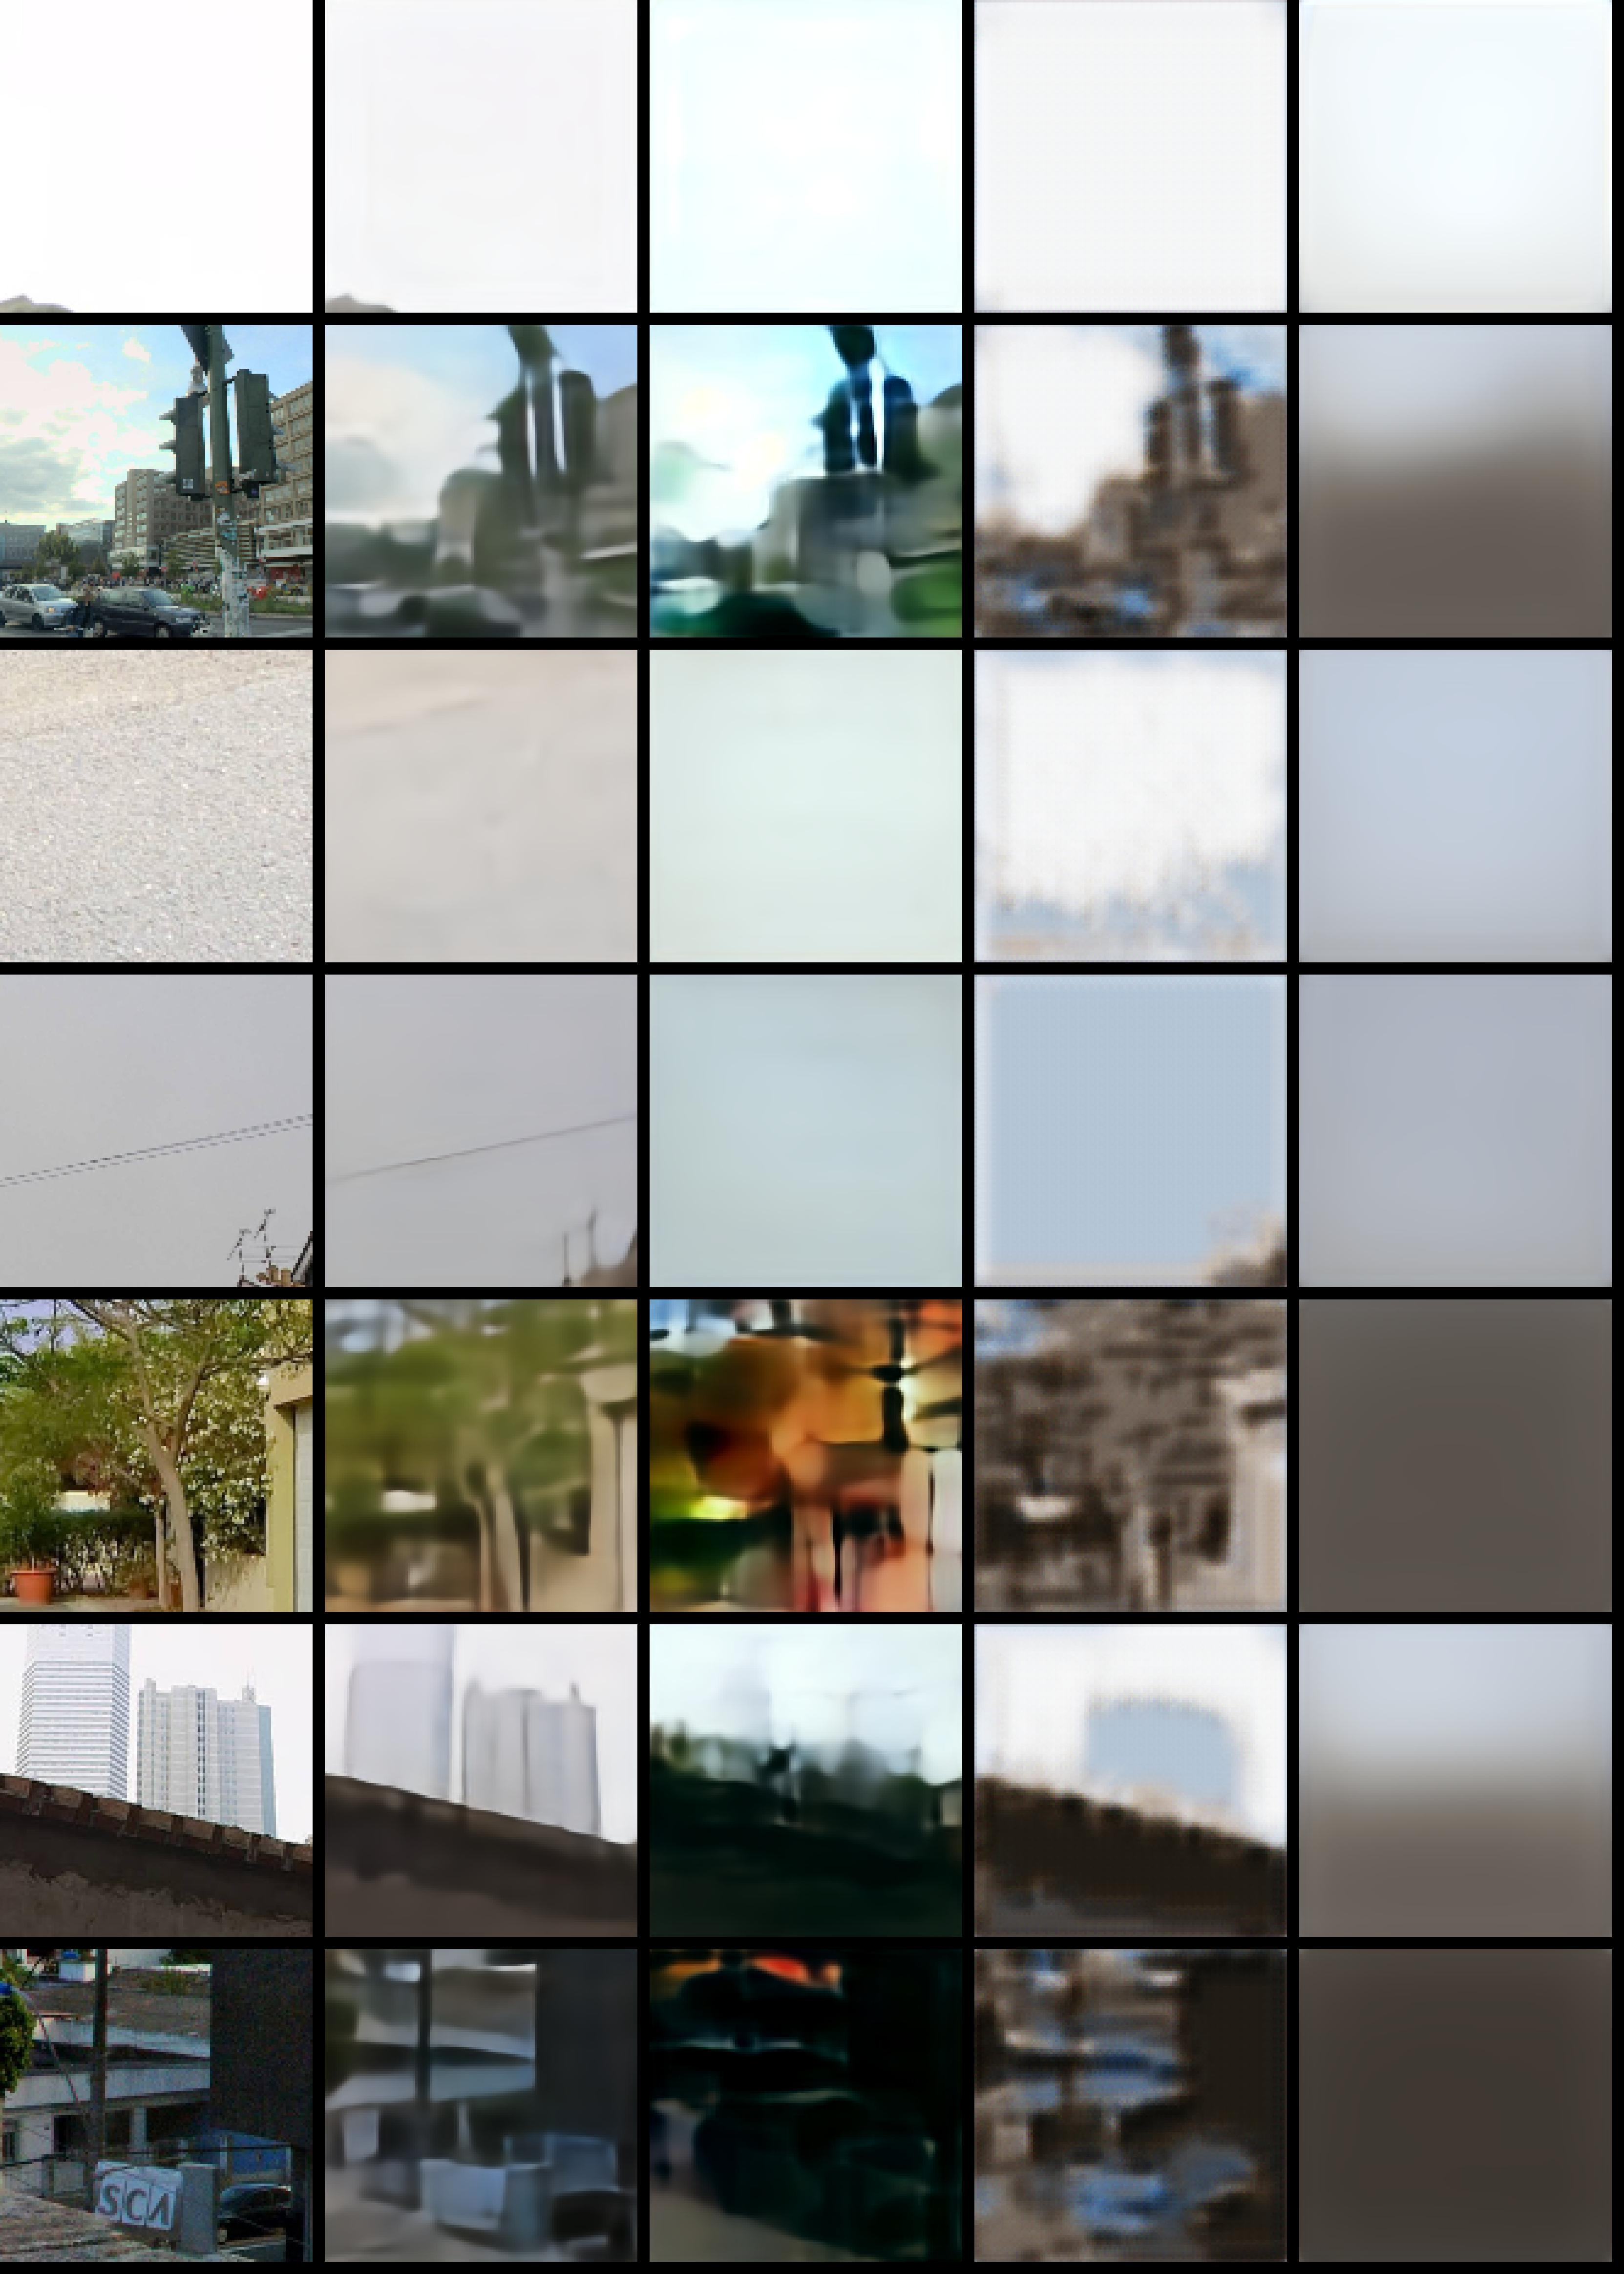
\includegraphics[width=0.92\textwidth]{figures/ptz/train_stacked_1.png}
\end{figure}
\begin{figure}
    \centering
    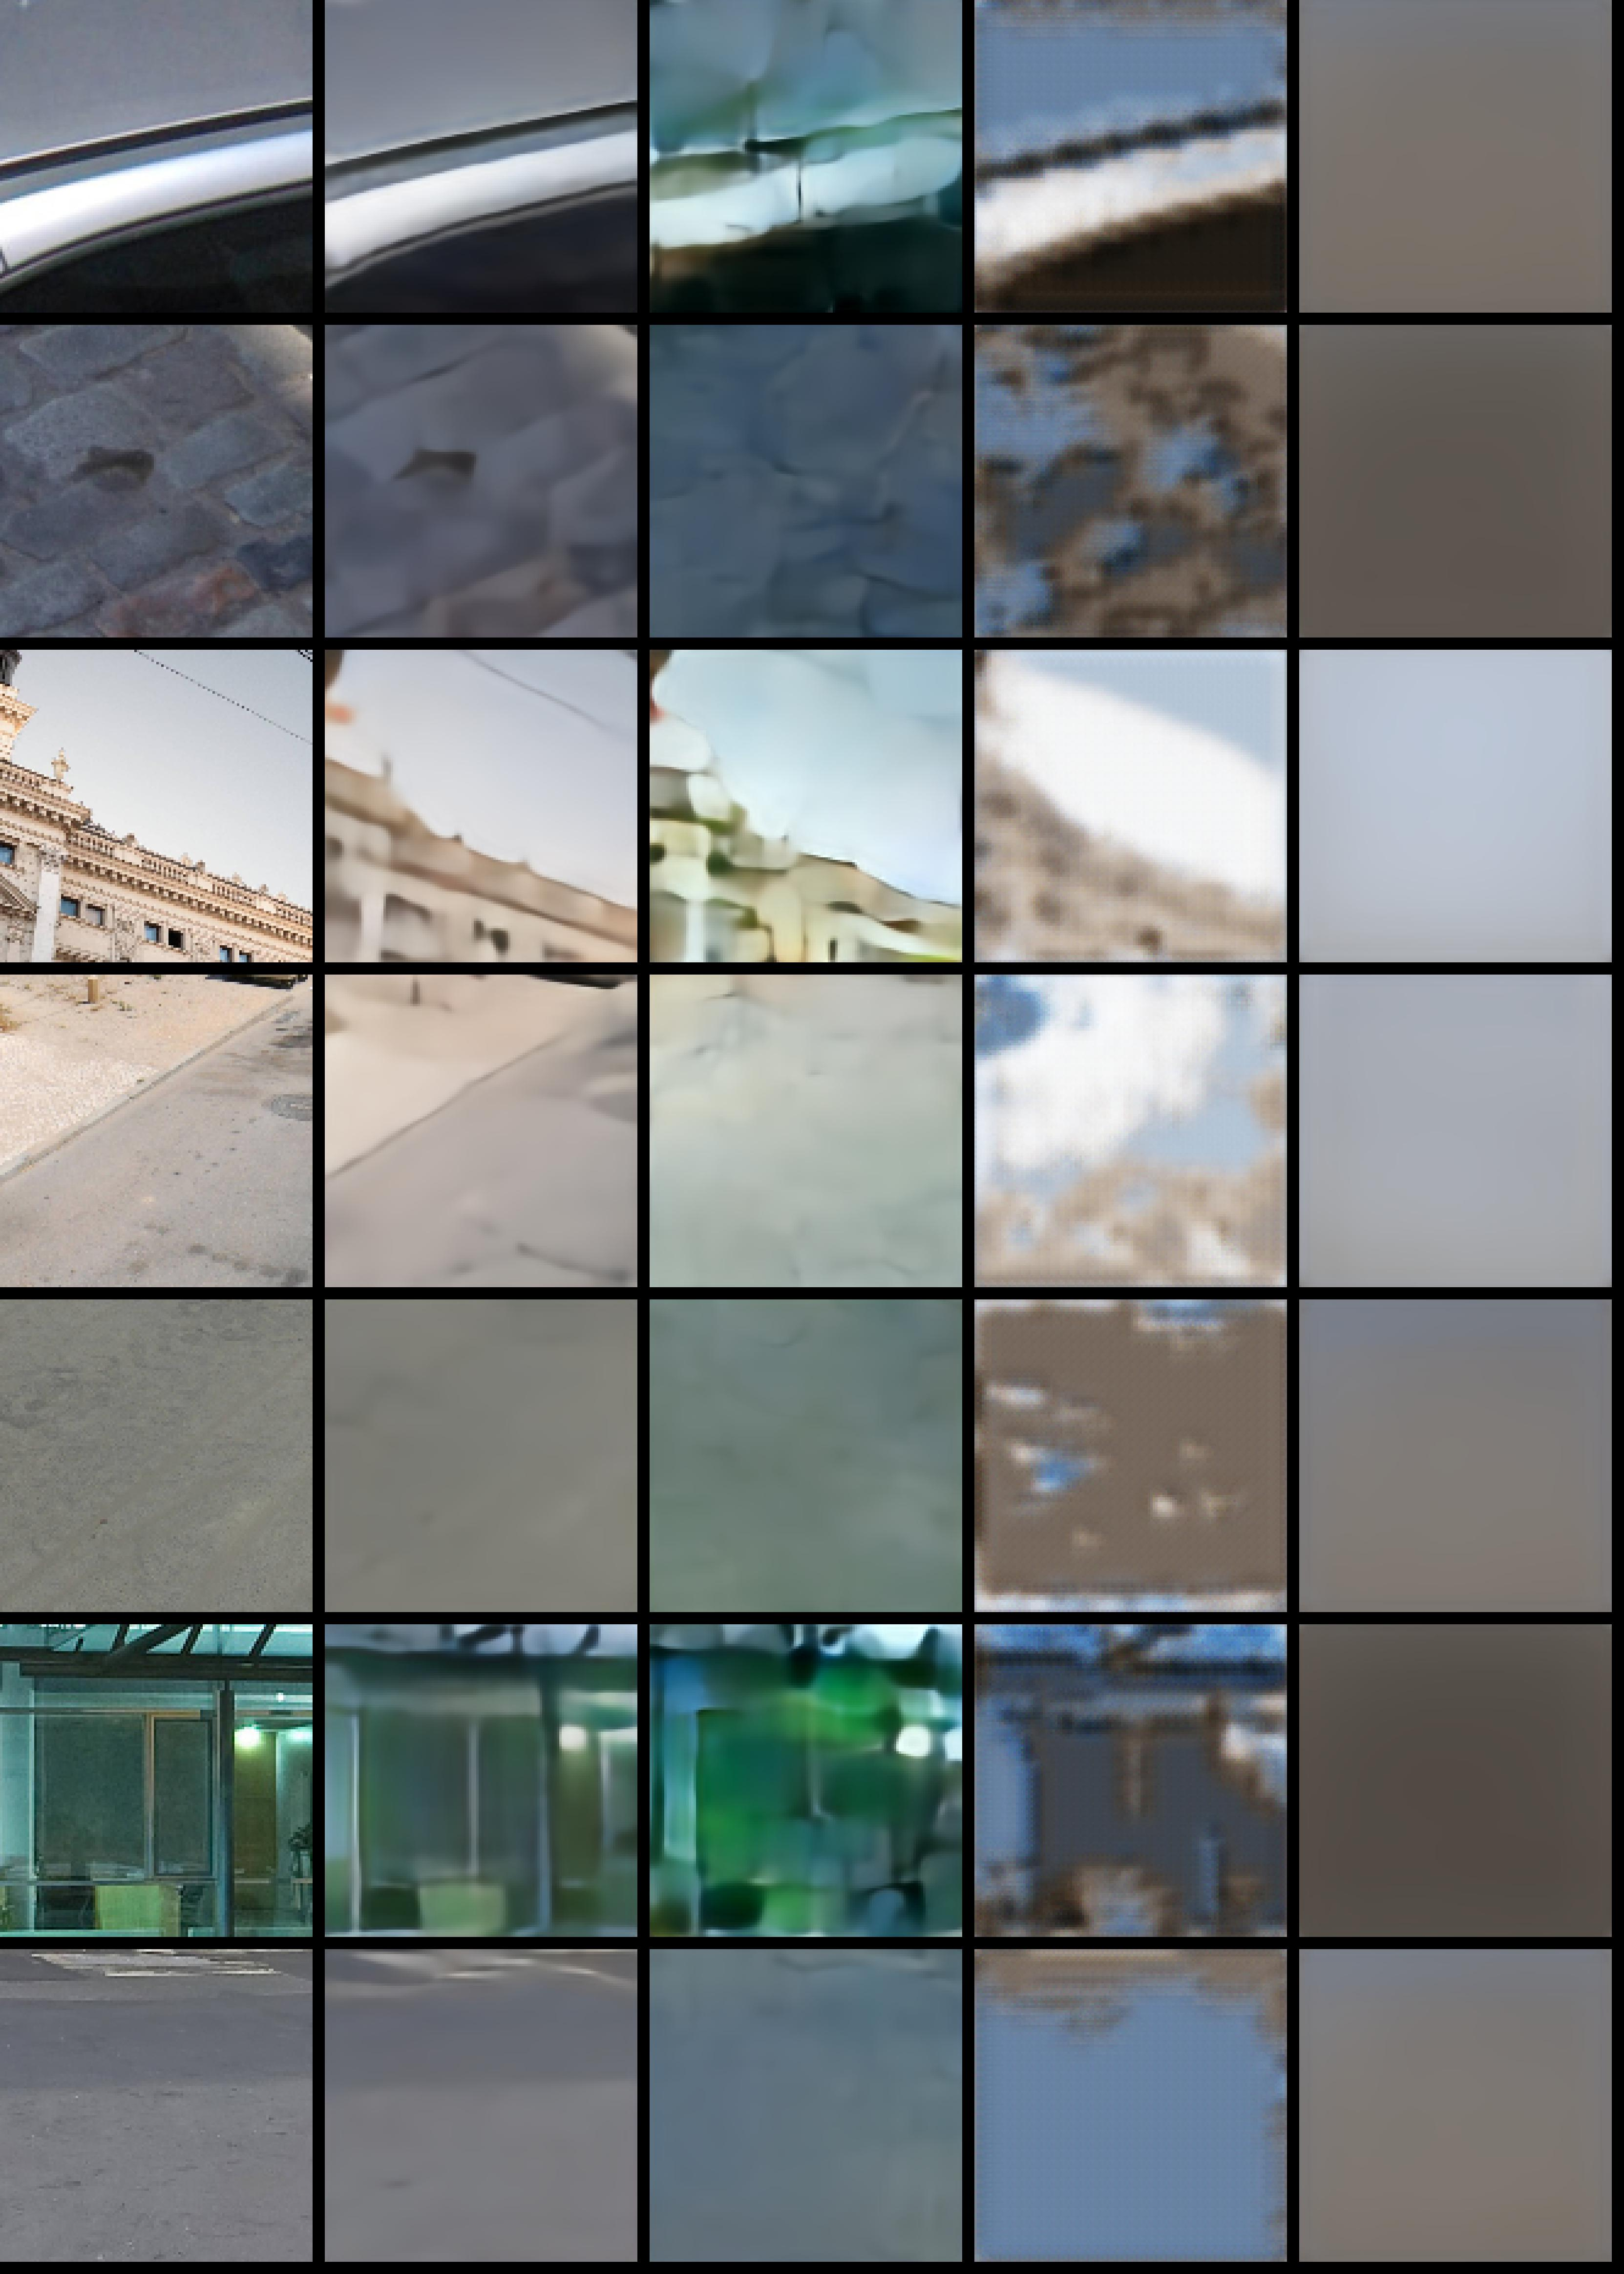
\includegraphics[width=0.92\textwidth]{figures/ptz/train_stacked_2.png}
\end{figure}
\begin{figure}
    \centering
    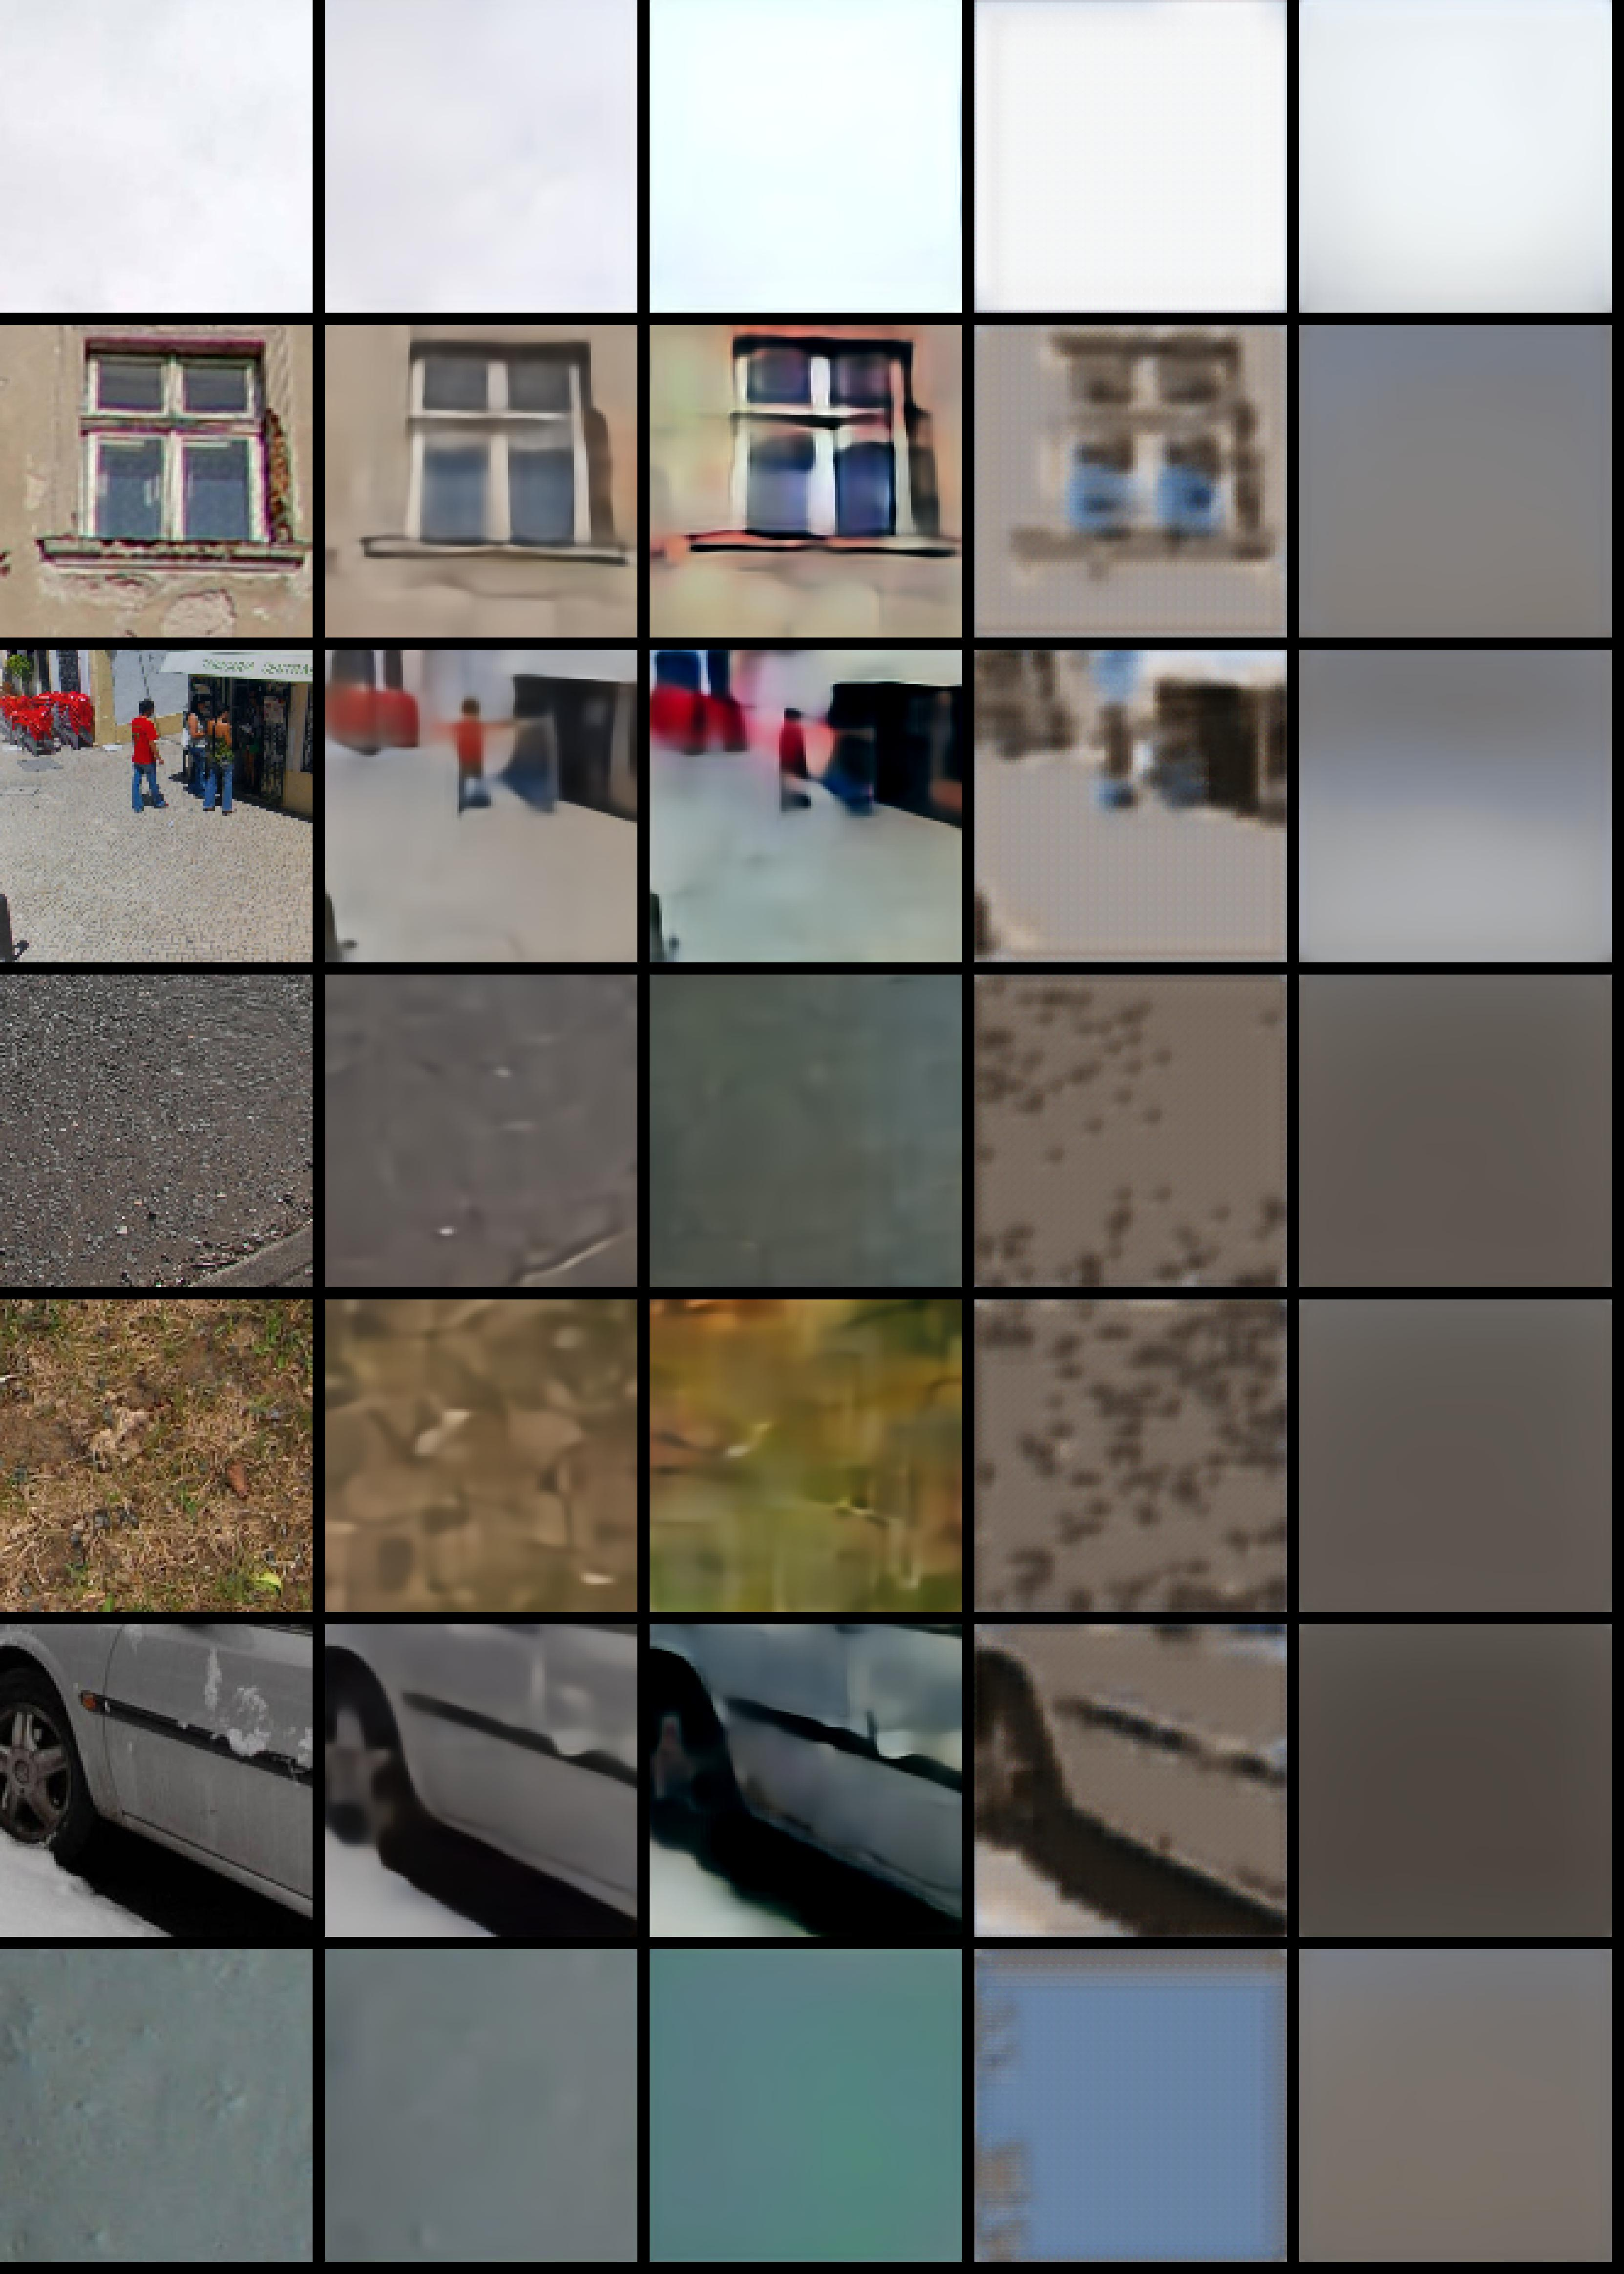
\includegraphics[width=0.92\textwidth]{figures/ptz/train_stacked_3.png}
\end{figure}
\begin{figure}
    \centering
    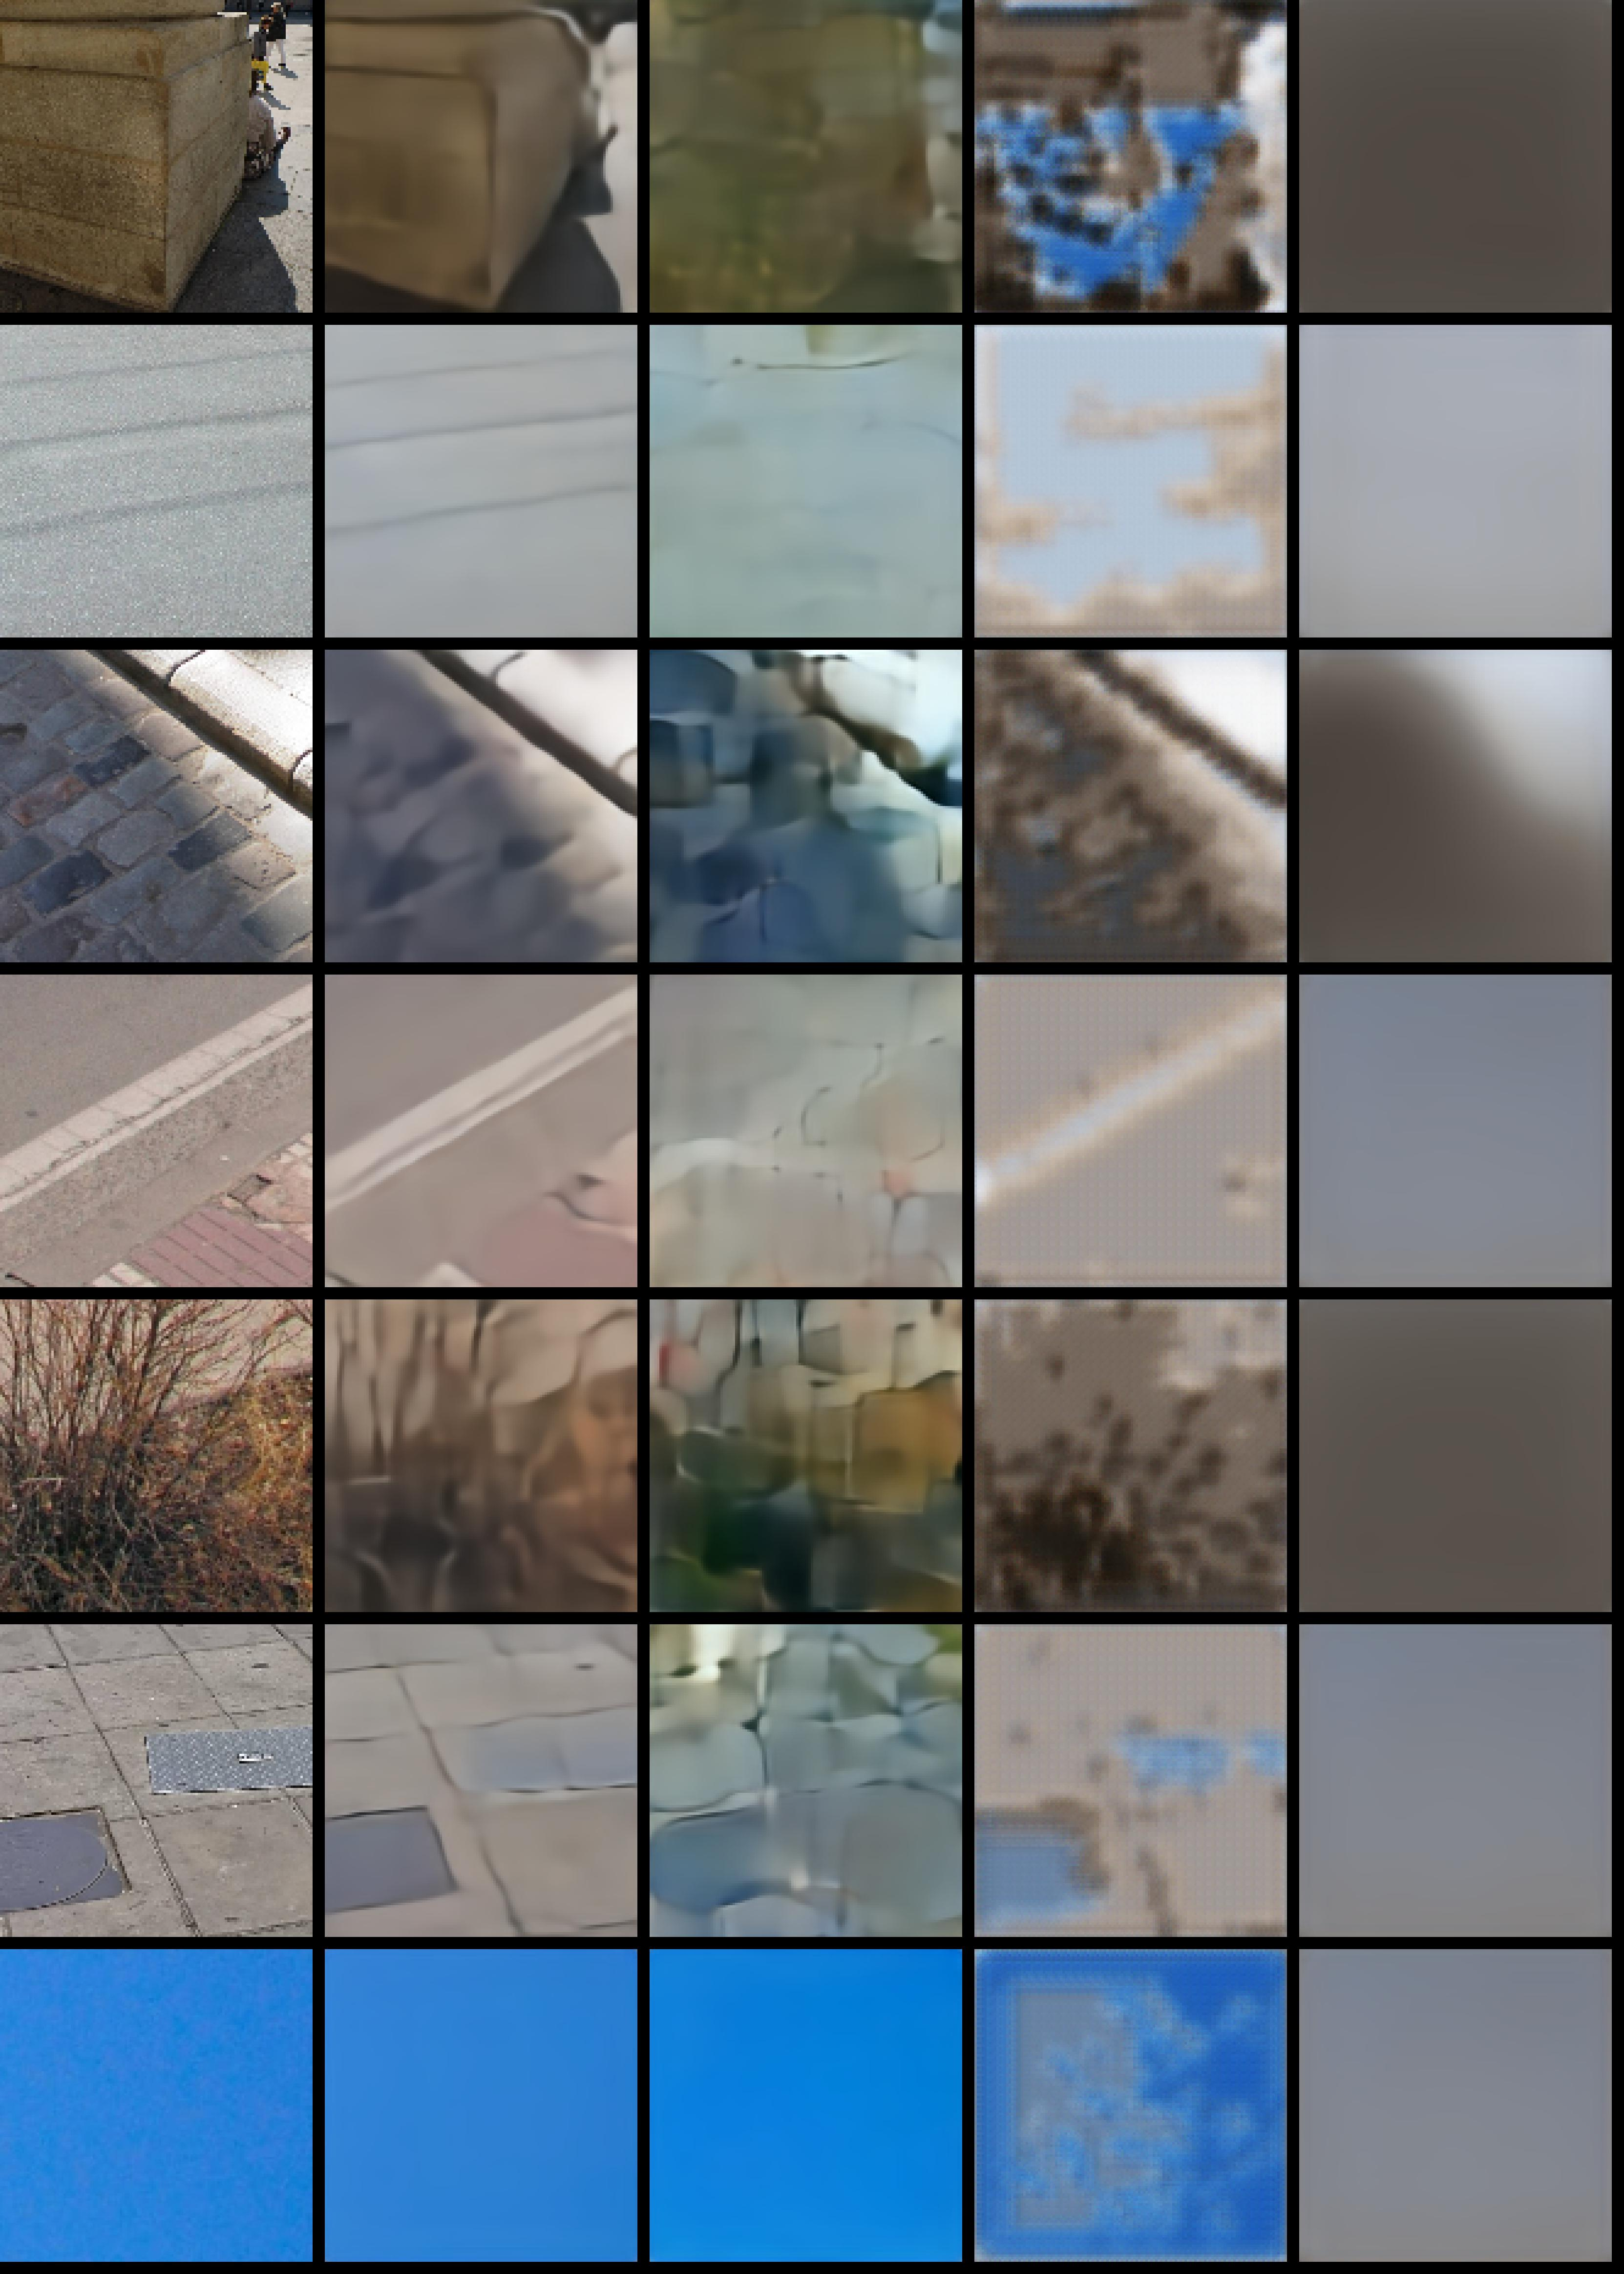
\includegraphics[width=0.92\textwidth]{figures/ptz/train_stacked_4.png}
\end{figure}

\begin{figure}
    \centering
    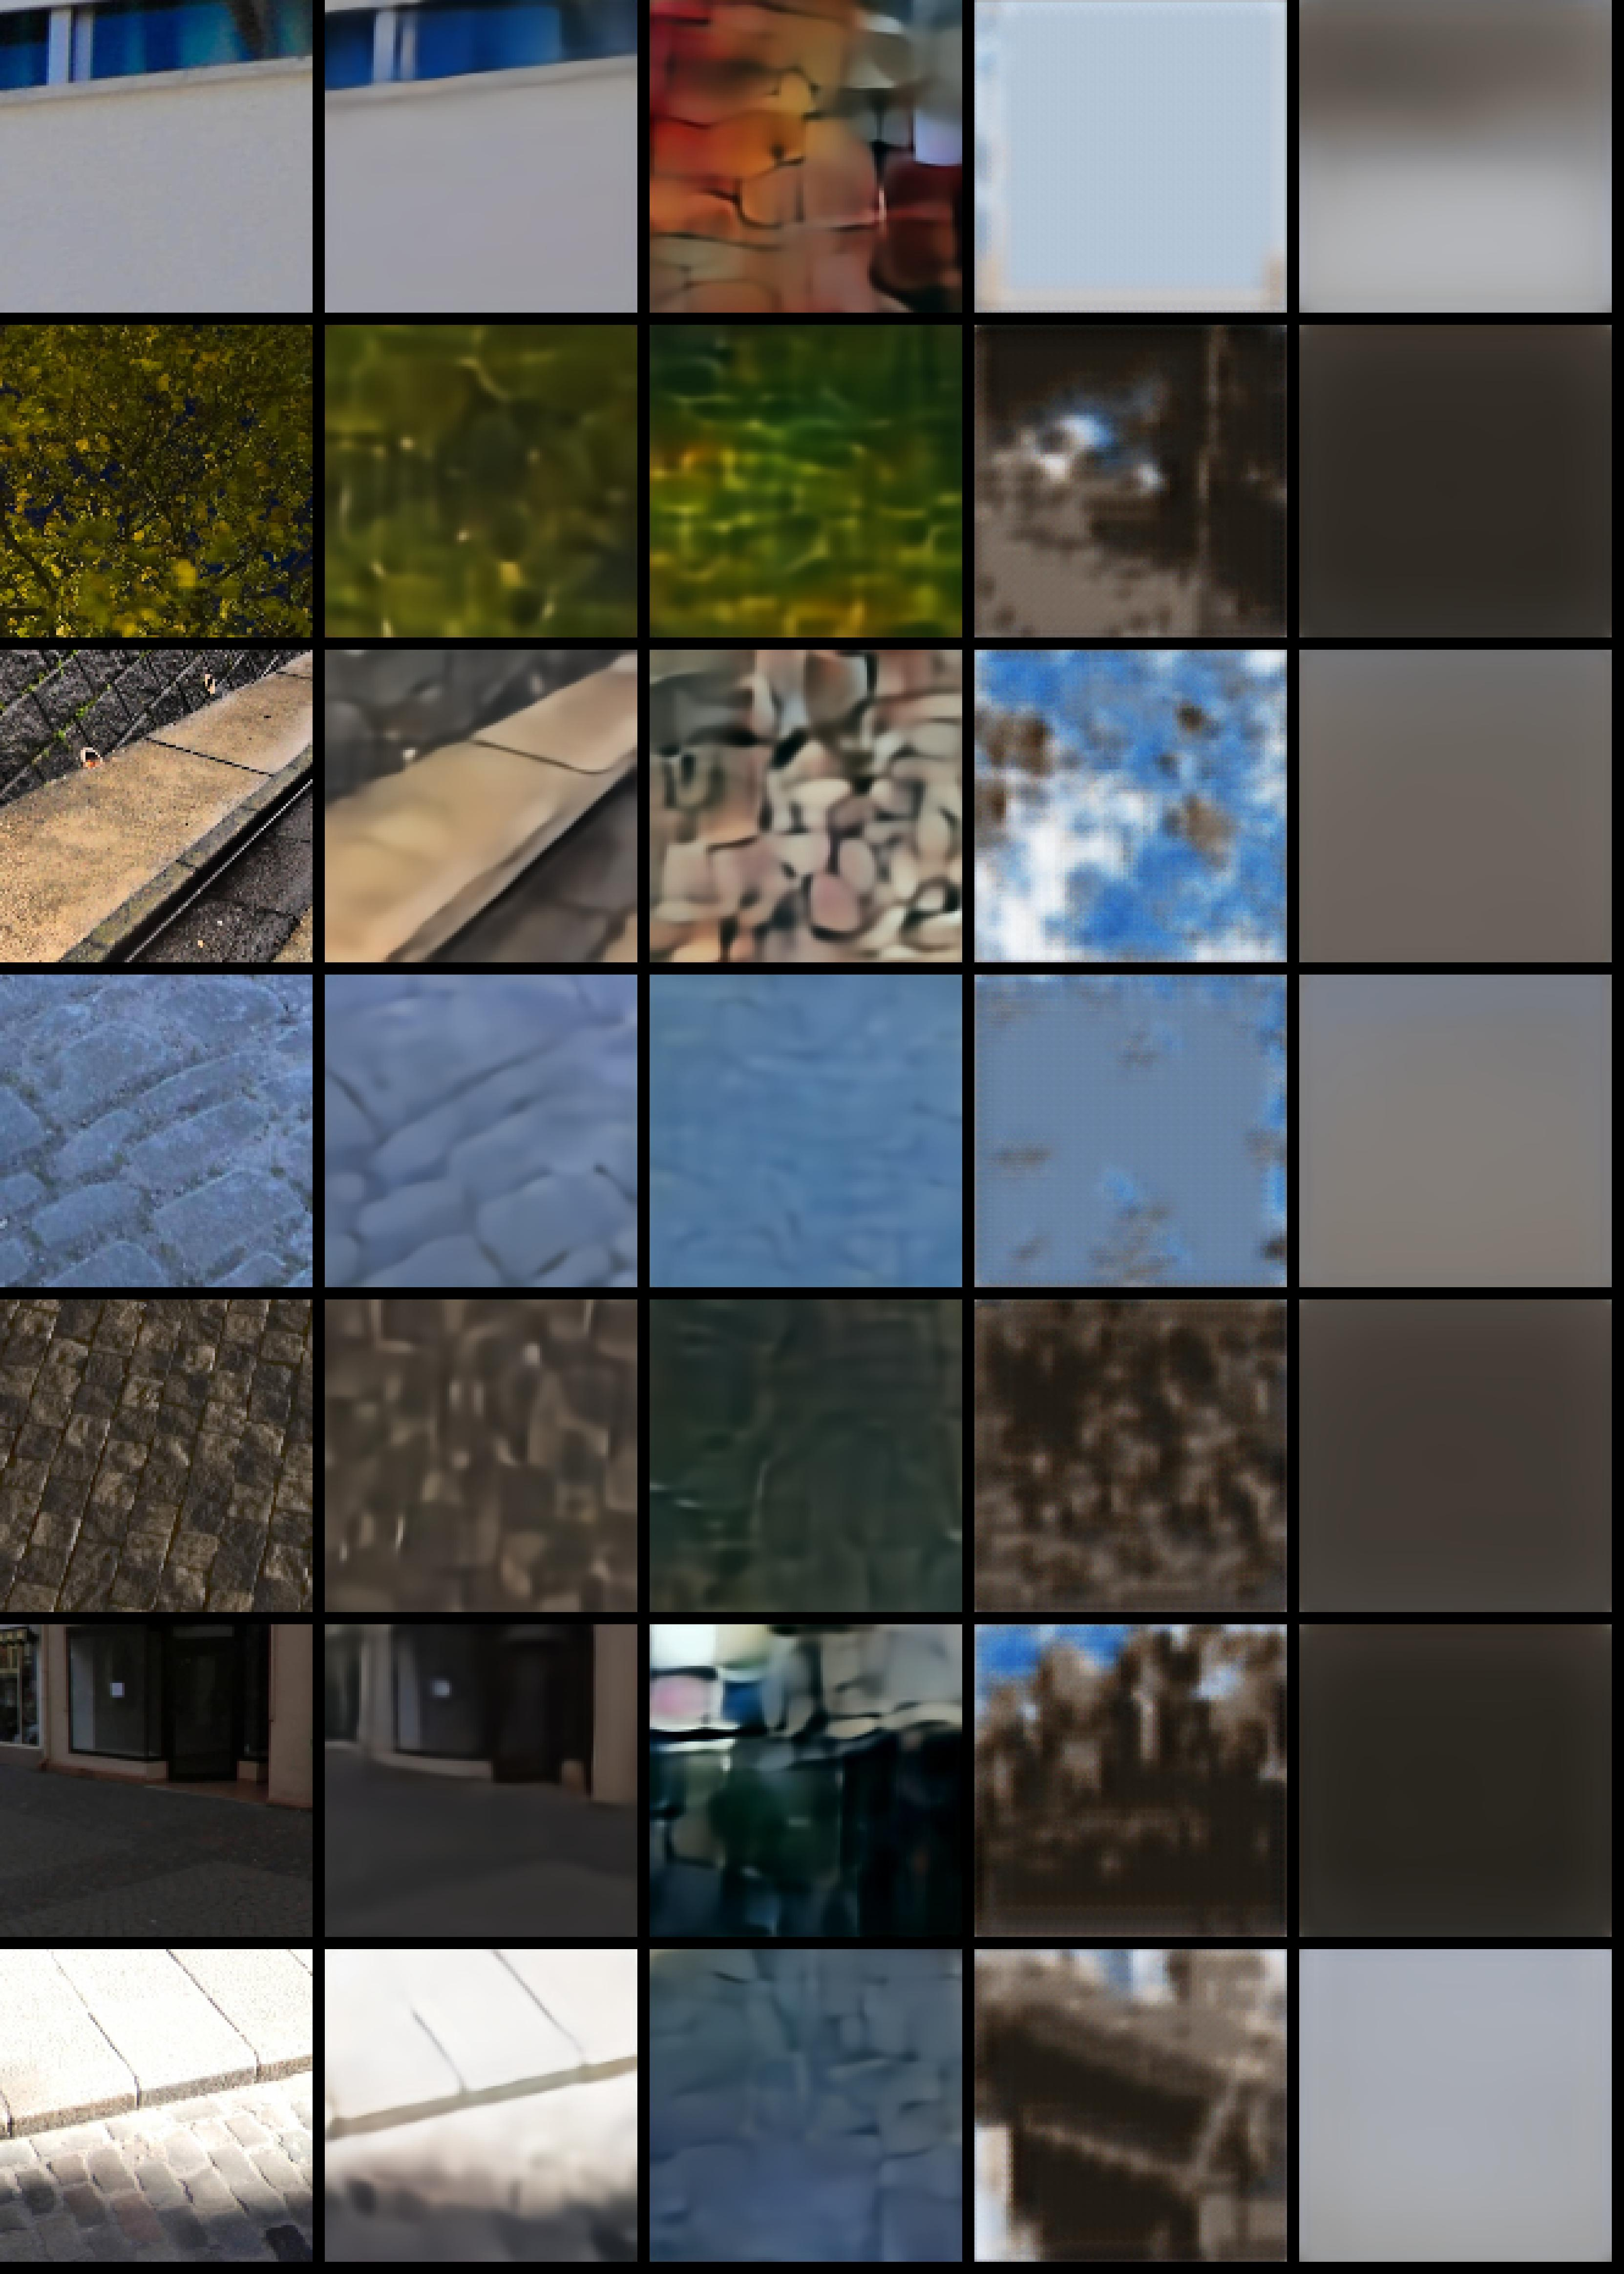
\includegraphics[width=0.92\textwidth]{figures/ptz/test_stacked_0.png}
\end{figure}
\begin{figure}
    \centering
    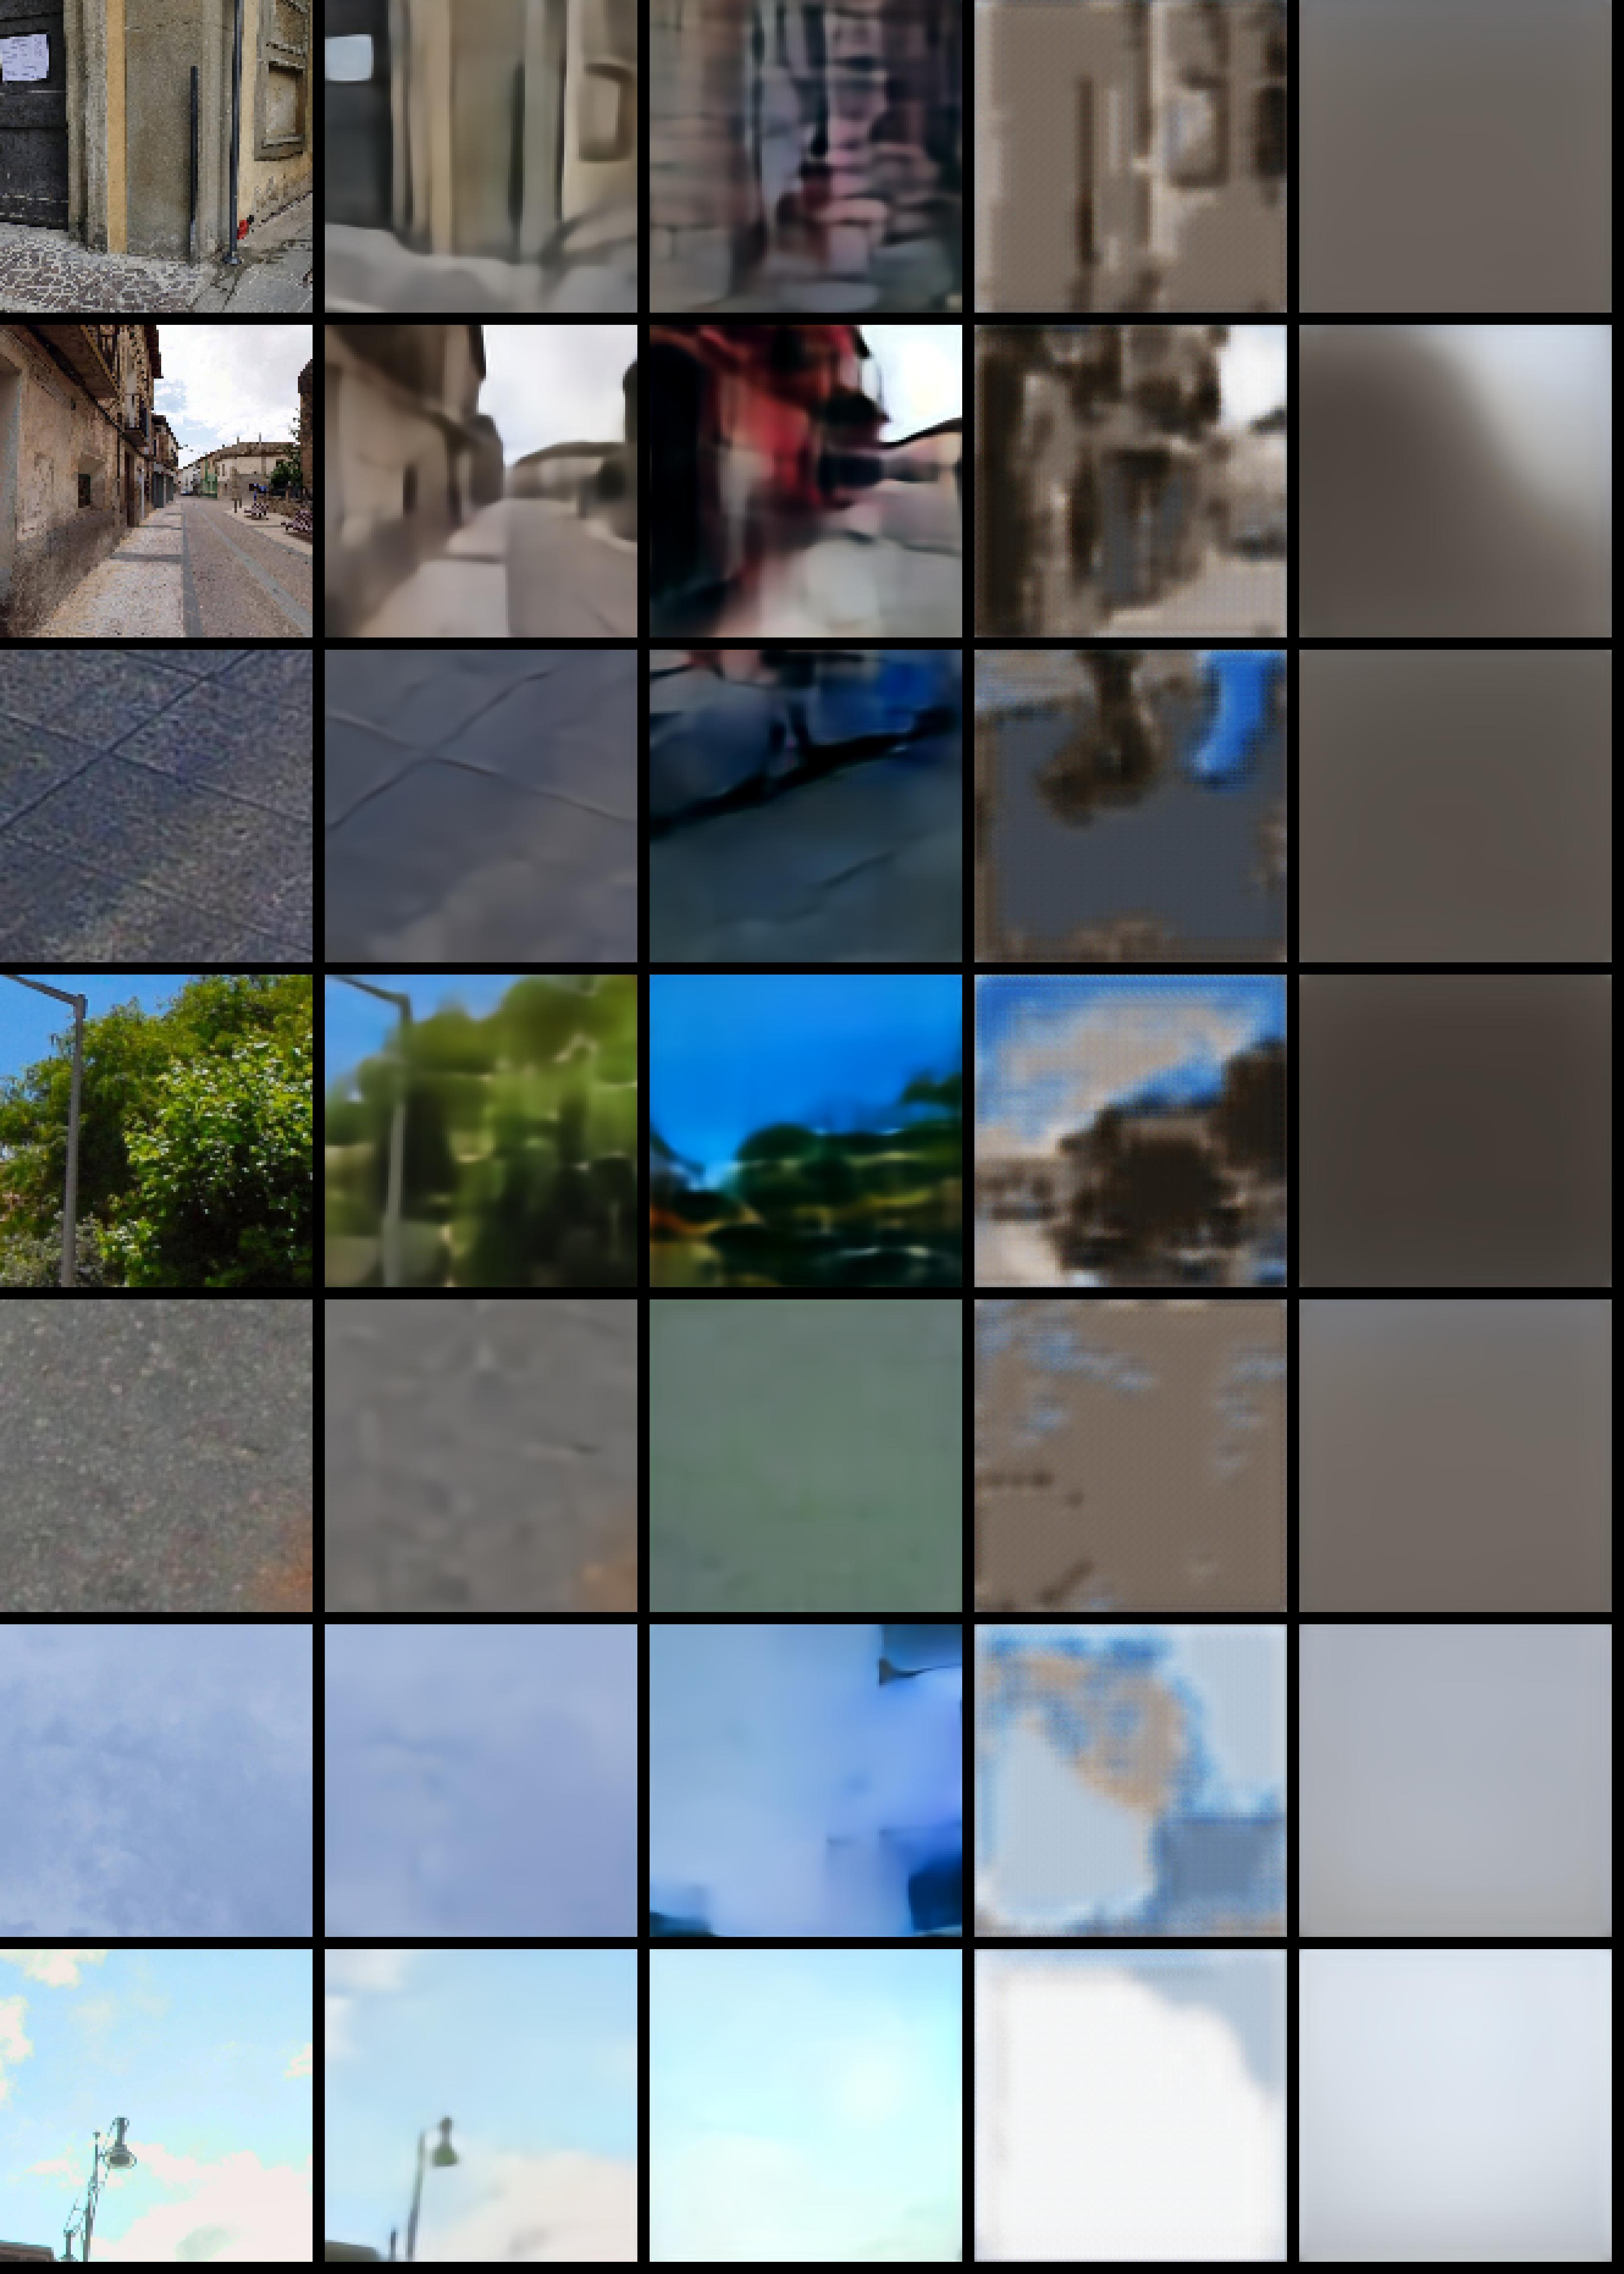
\includegraphics[width=0.92\textwidth]{figures/ptz/test_stacked_1.png}
\end{figure}
\begin{figure}
    \centering
    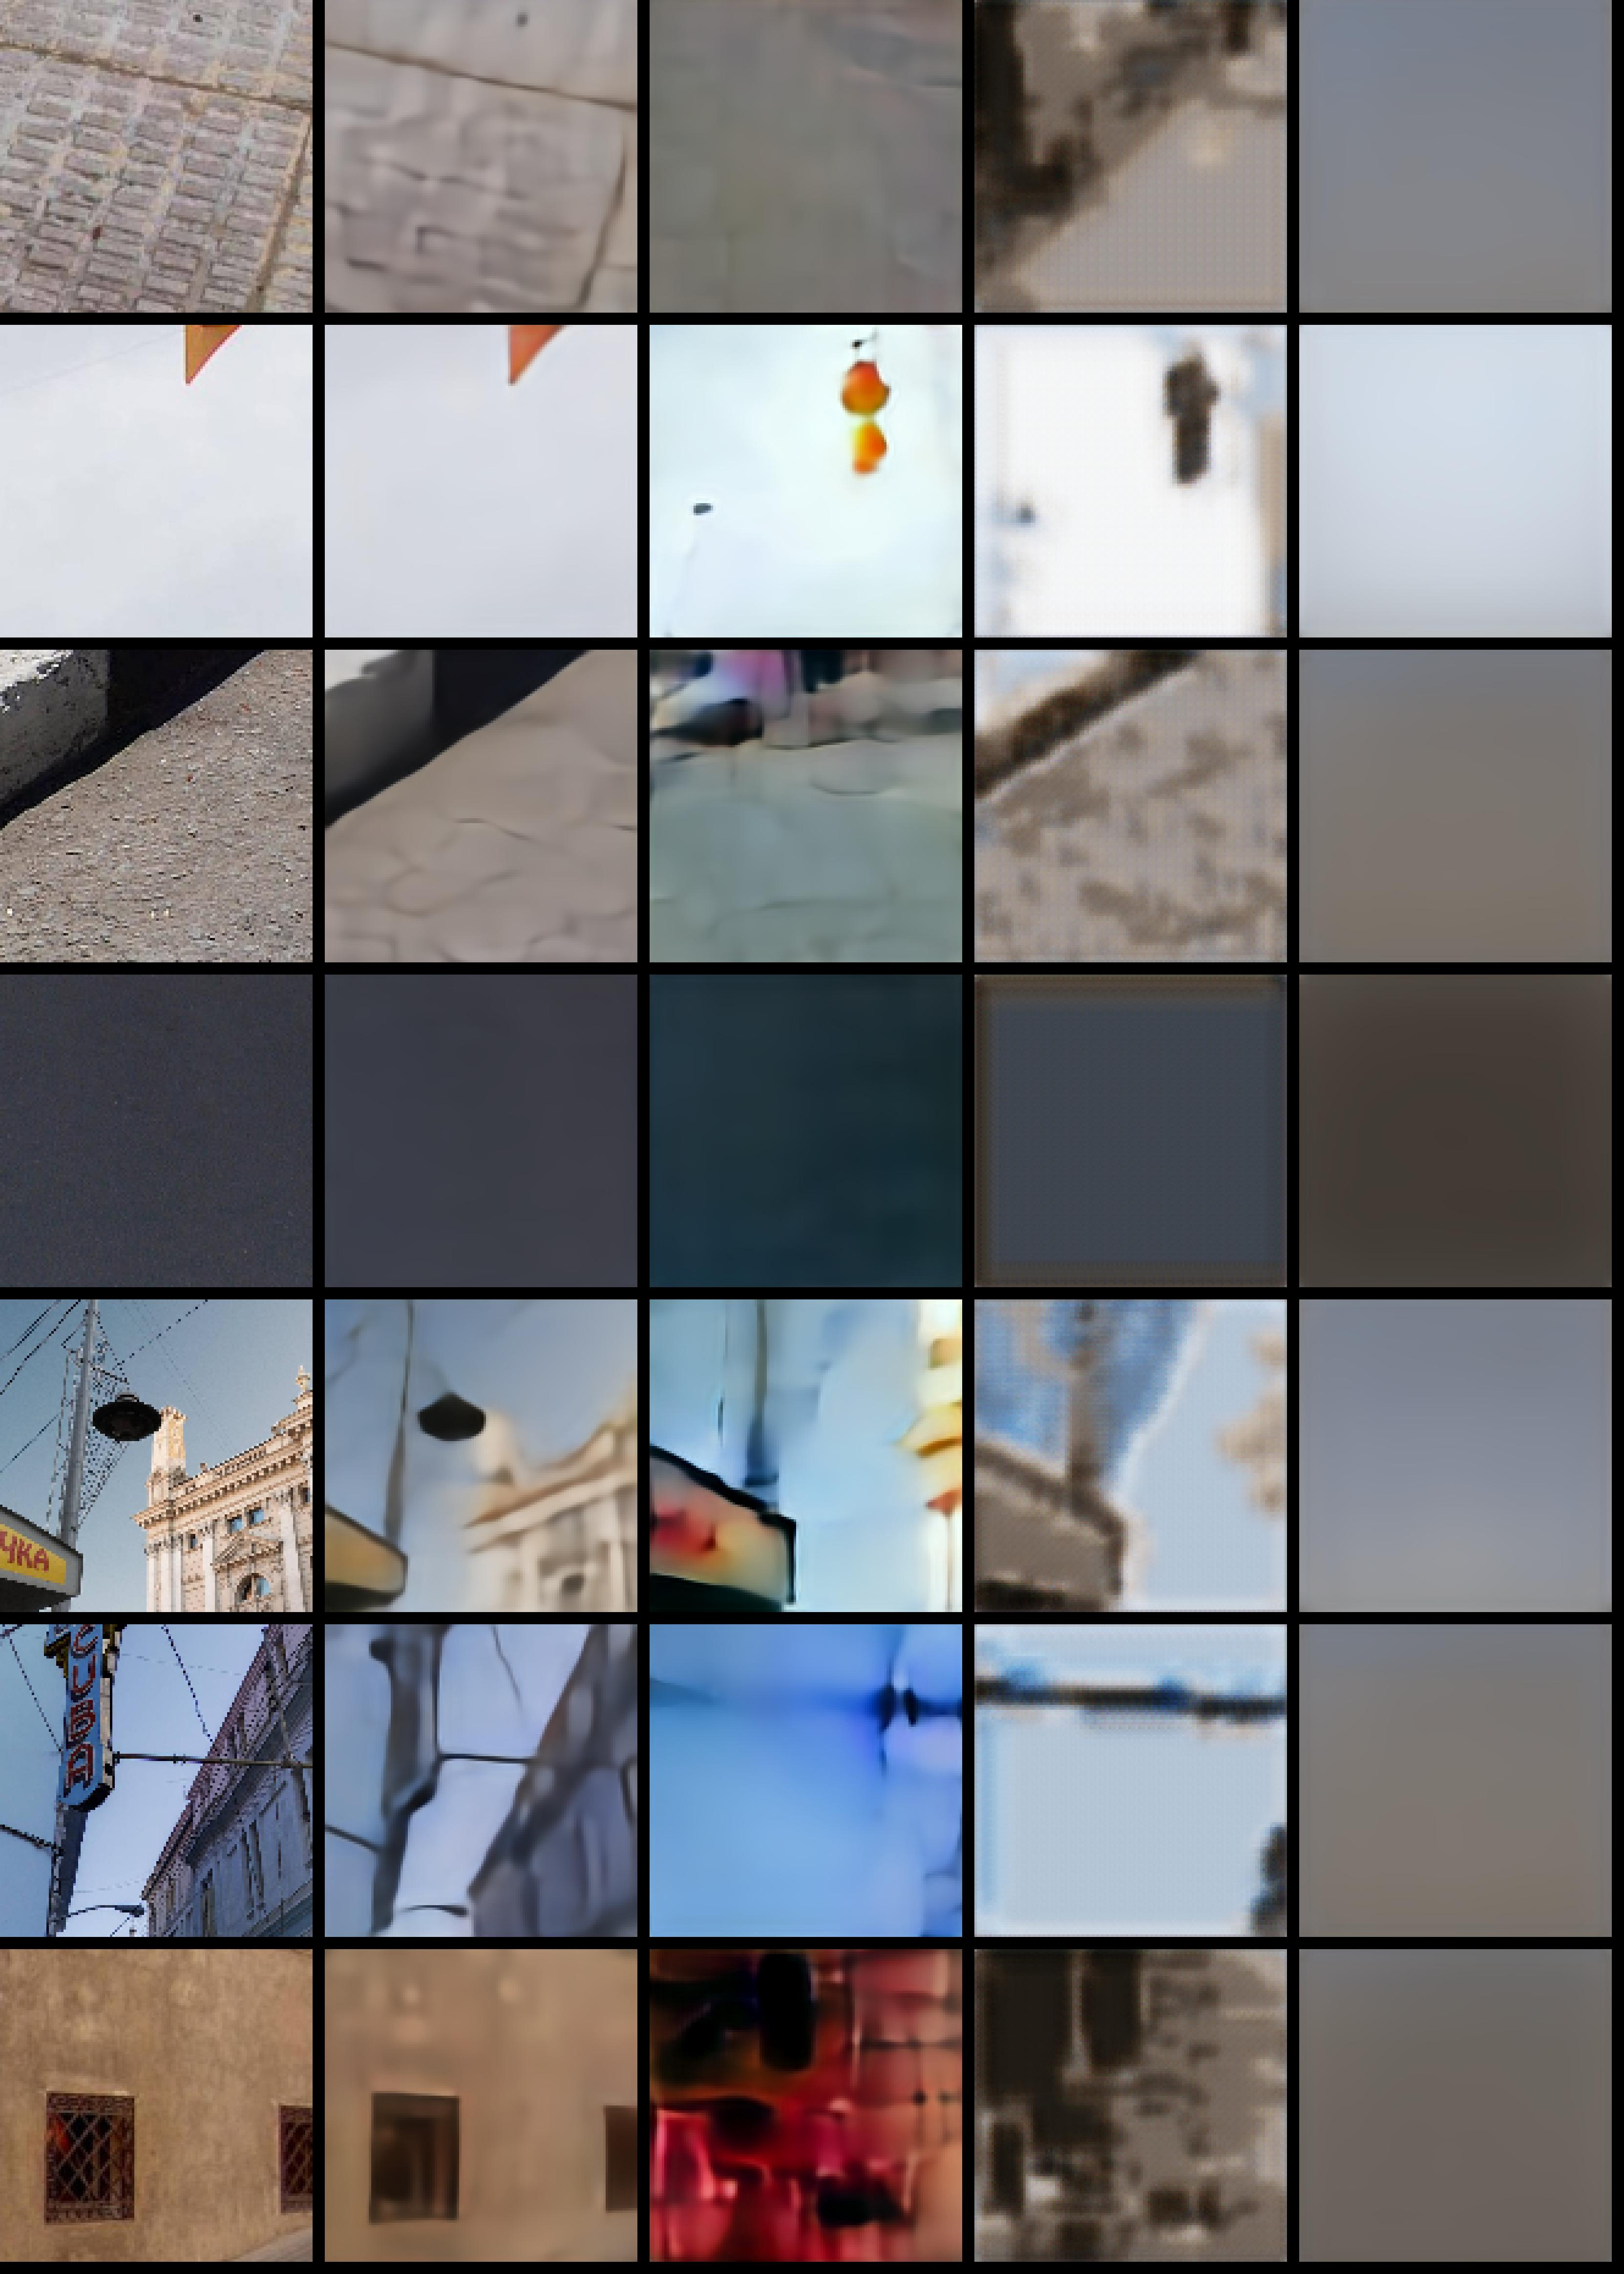
\includegraphics[width=0.92\textwidth]{figures/ptz/test_stacked_2.png}
\end{figure}
\begin{figure}
    \centering
    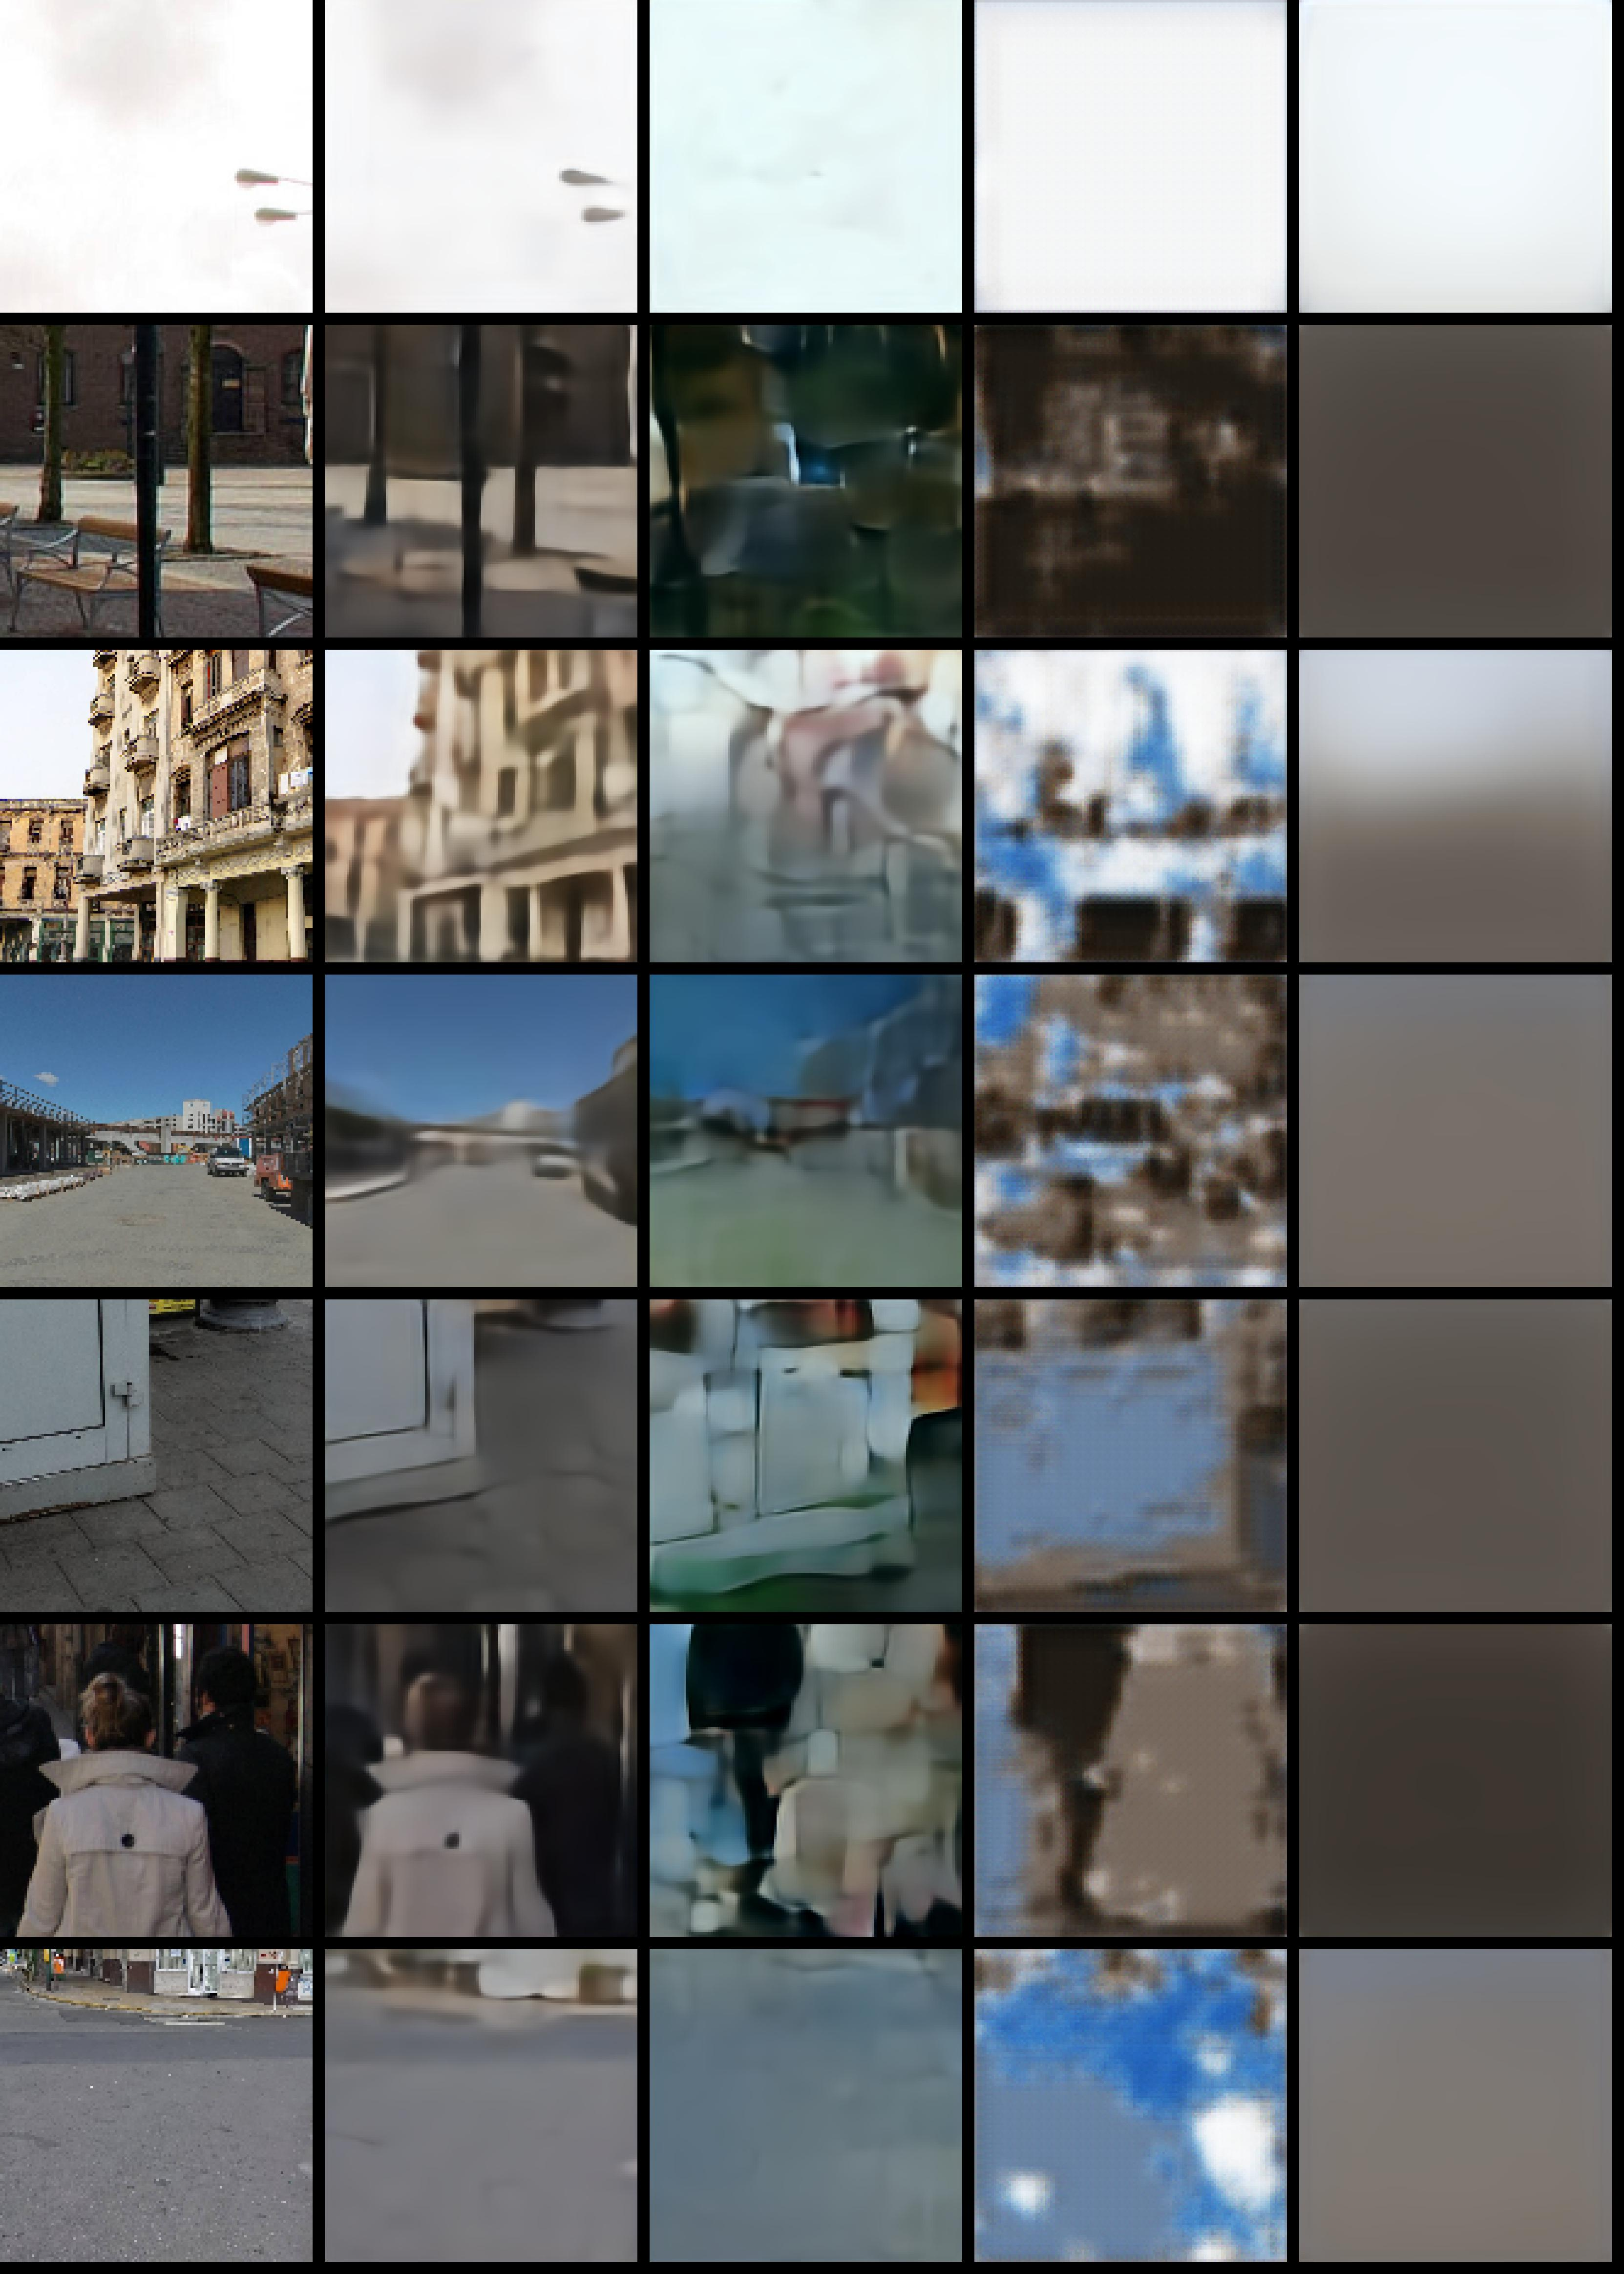
\includegraphics[width=0.92\textwidth]{figures/ptz/test_stacked_3.png}
\end{figure}
\begin{figure}
    \centering
    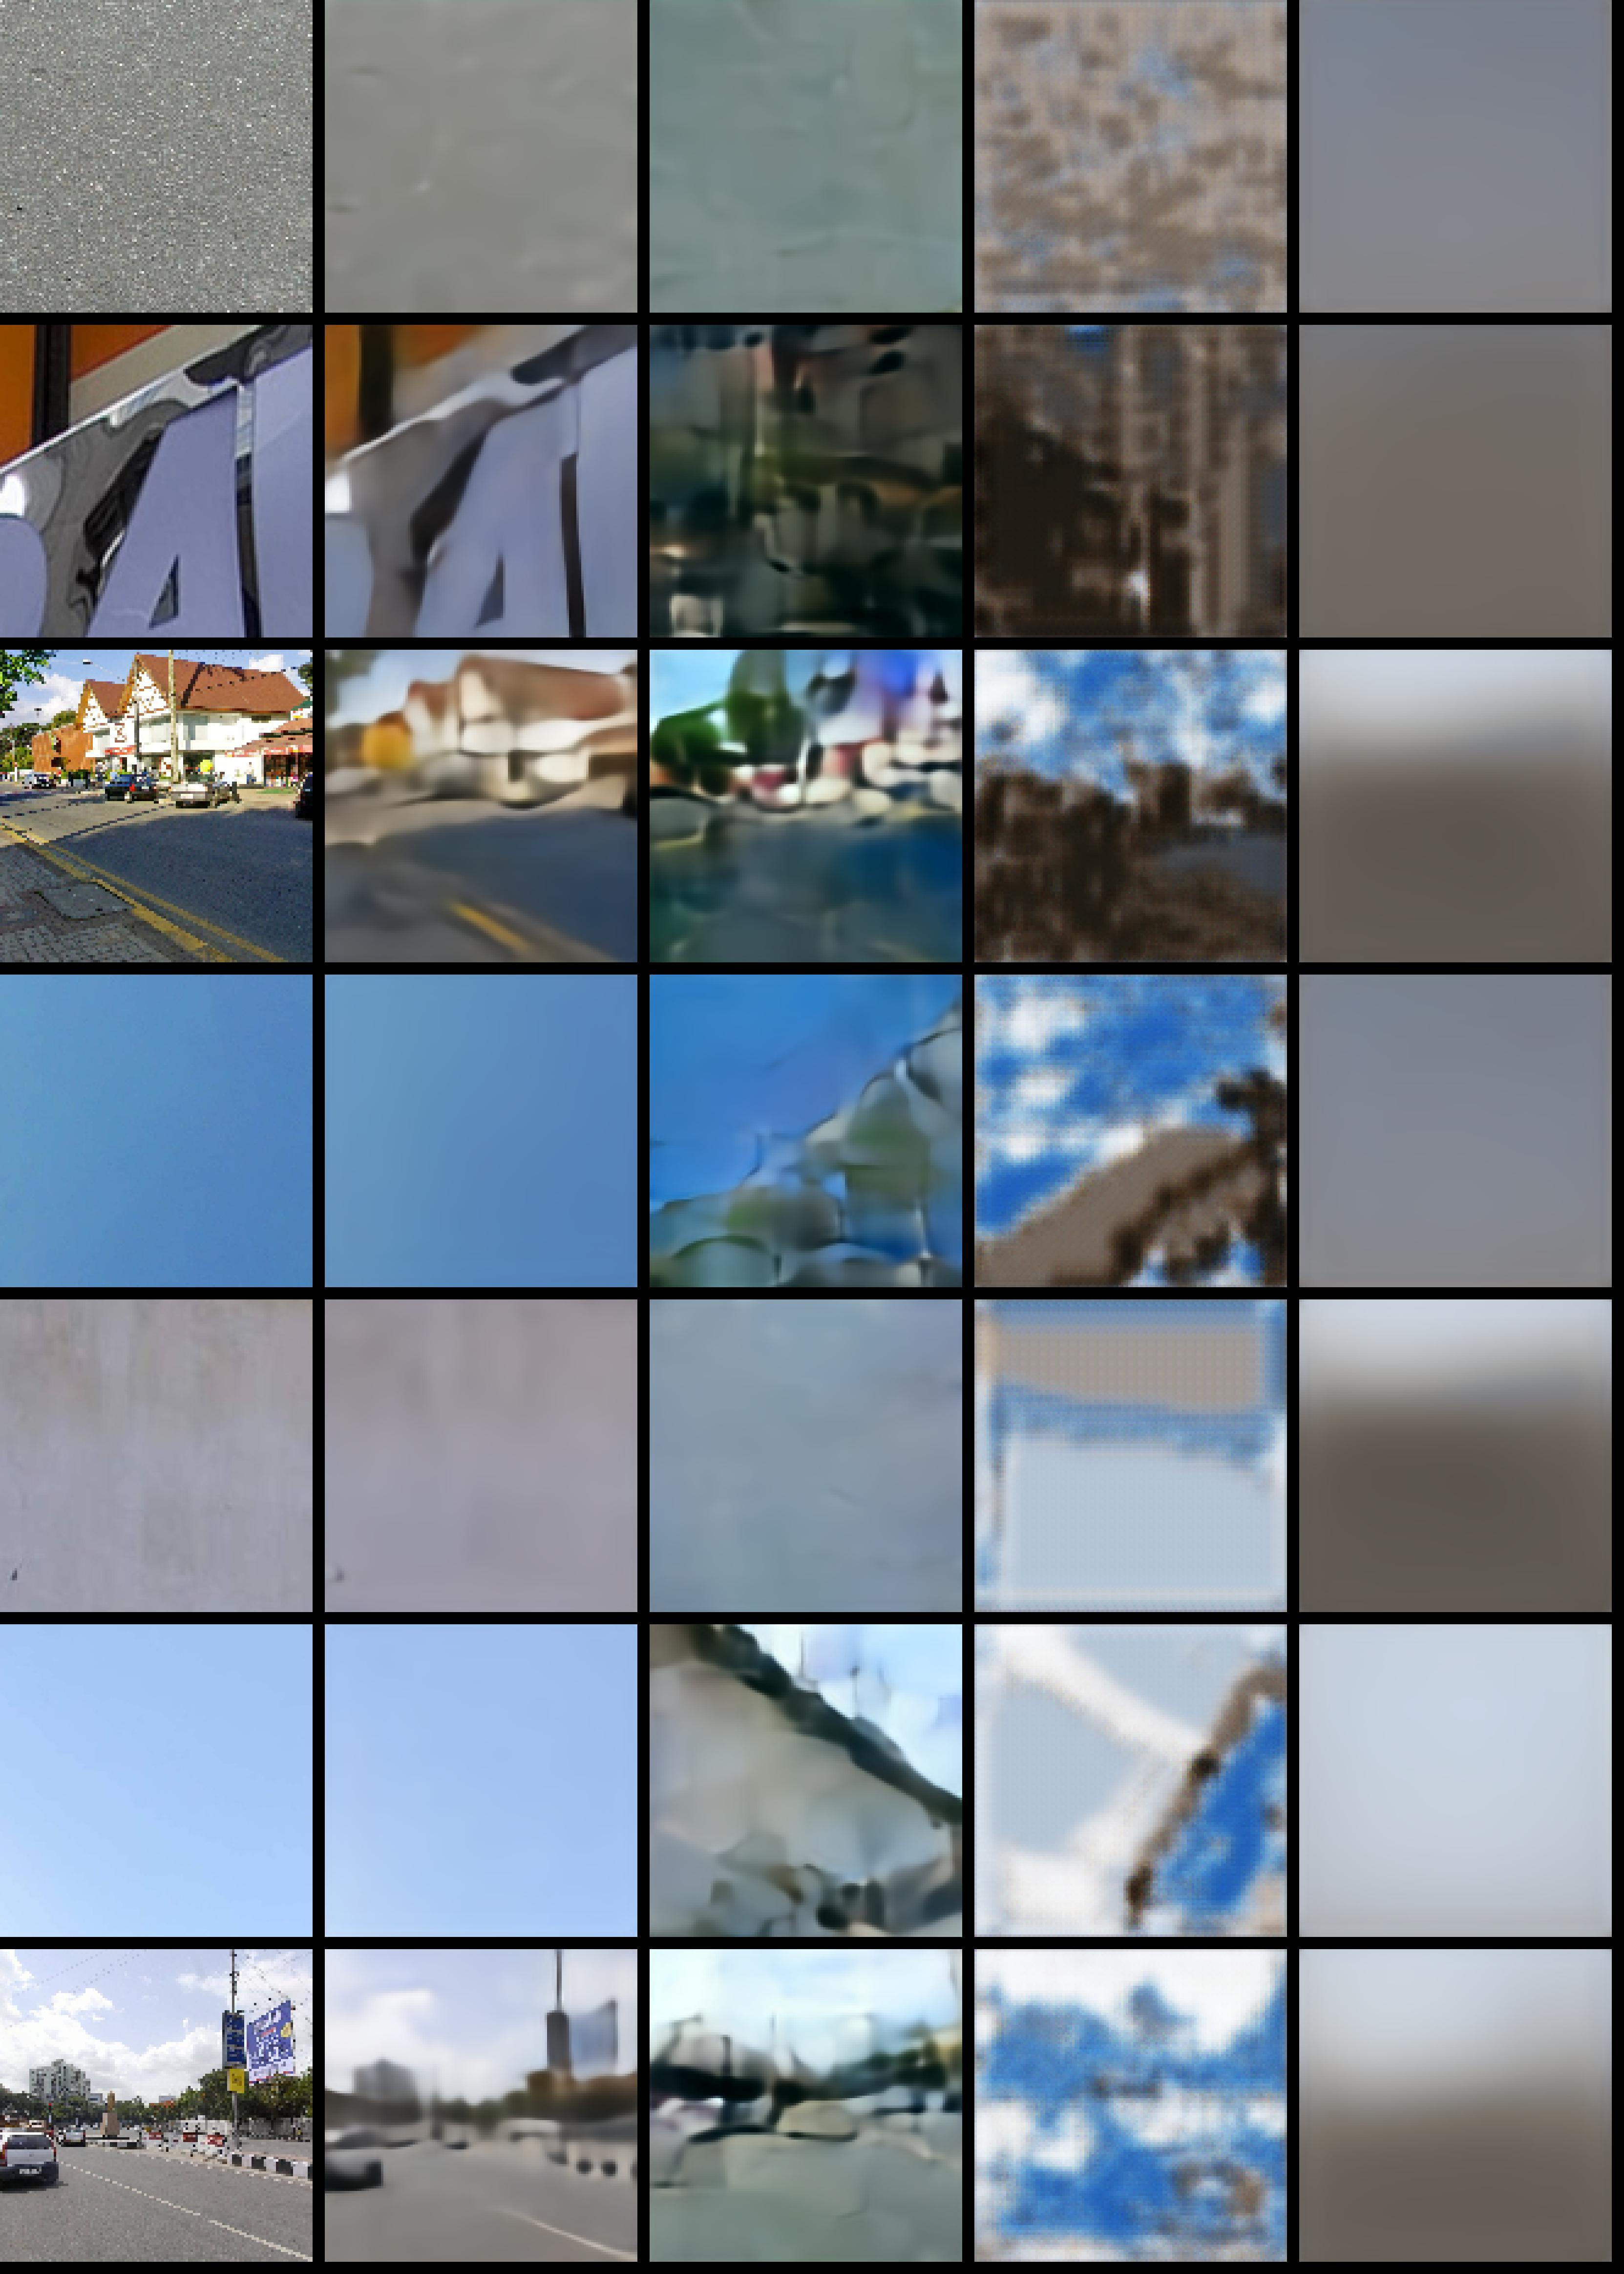
\includegraphics[width=0.92\textwidth]{figures/ptz/test_stacked_4.png}
\end{figure}

\end{appendices}